\documentclass[a4paper,12pt]{article}
\usepackage{geometry}
\geometry{left=2.5cm,right=2.5cm,top=2.5cm,bottom=2.5cm}
\usepackage{ctex}  
\usepackage{graphicx}
\usepackage{fancyhdr}
\usepackage{array}
\usepackage{titlesec}
\usepackage{amsmath}
\usepackage{caption}
\usepackage{booktabs}
\usepackage{makecell}
\usepackage{subcaption} 

\usepackage{listings}
\usepackage{xcolor}
\usepackage{geometry}
\usepackage[section]{placeins}
\definecolor{codegreen}{rgb}{0,0.6,0}
\definecolor{codegray}{rgb}{0.5,0.5,0.5}
\definecolor{codepurple}{rgb}{0.58,0,0.82}
\definecolor{backcolour}{rgb}{0.95,0.95,0.92}

\lstdefinestyle{mystyle}{
	backgroundcolor=\color{backcolour},   
	commentstyle=\color{codegreen},
	keywordstyle=\color{magenta},
	numberstyle=\tiny\color{codegray},
	stringstyle=\color{codepurple},
	basicstyle=\ttfamily\footnotesize,
	breakatwhitespace=false,         
	breaklines=true,                 
	captionpos=b,                    
	keepspaces=true,                 
	numbers=left,                    
	numbersep=5pt,                  
	showspaces=false,                
	showstringspaces=false,
	showtabs=false,                  
	tabsize=2,
	frame=single
}

\lstset{style=mystyle}


\pagestyle{fancy}
\fancyhf{}
\cfoot{\thepage}
\renewcommand{\headrulewidth}{0pt} %禁用页眉线


% 设置标题格式
\titleformat{\section}{\centering\bfseries\zihao{4}}{\thesection}{1em}{}

\begin{document}
	
	% 封面页
	\begin{titlepage}
		
		\vspace{0.677cm}
		
		\begin{flushright}
			\begin{tabular}{|m{3cm}|m{3cm}|}
				\hline
				\songti \zihao{4} 参赛编号 & \hspace{2cm} \\
				\hline
				\multicolumn{2}{c}{\lishu \zihao{4} \hspace*{2cm} (由组委会填写)} \\
			\end{tabular}
		\end{flushright}
		
		\vspace*{2.8cm}

		{
			\centering
			
\includegraphics[width=0.5\textwidth]{南京信息工程大学.png}
			
			\vspace{1cm}
			
			{\zihao{1} \textbf{第十九届数学建模竞赛论文}}
			
			\vspace{2cm}
			
			{\heiti \zihao{3} \textbf{选题:A题\ 江苏省空气质量综合指数建模与预测分析}}
			
			\vspace{2cm}
		}
		
		{\heiti \zihao{3} \textbf{参赛队员:}}
		
		\centering
		
		\vspace{0.5cm}
		
		\begin{center}
			\songti \zihao{4}
			\begin{tabular}{|m{3cm}|m{4cm}|m{4cm}|m{4cm}|}
				\hline
				姓名 & 学院 & 学号 & 专业 \\
				\hline
				队长 & 王晨屹&202383270216 &电子信息工程 \\
				\hline
				队员 1 &丁诚诚 &202383290102 &计算机科学与技术 \\
				\hline
				队员 2 & 梅应宝&202383290121 &计算机科学与技术 \\
				\hline
			\end{tabular}
		\end{center}
		
		\vfill
		
		{\heiti \zihao{4} 二〇二五年五月}
		
	\end{titlepage}
	
	% 摘要页
	\newpage
	\setcounter{page}{1}
	
	\begin{center}
		
\includegraphics[width=0.4\textwidth]{南京信息工程大学.png}
	\end{center}
	
	
	\begin{center}
		\textbf{\zihao{1} 第十九届数学建模竞赛}
	\end{center}
	
	\vspace{0.593cm}
	
	\begin{center}
		\heiti \zihao{4}\textbf{论文题目:江苏省空气质量综合指数建模及区域协同治理研究\hspace{2cm}}
	\end{center}
	
	\begin{center}
		\lishu	\zihao{2}\textbf{摘\quad 要:}\\
	\end{center}

	
	
	{\zihao{5}
		
		本研究主要围绕江苏省空气质量综合指数的建模和预测分析展开,通过构建预测模型与评估区域关联性,旨在助力气象部门制定针对性的污染防治策略。
		
		\textbf{针对问题一:}设计缺失值填补方案与异常值查找方案,保证插入准确合理的数值,并分析两种插值方案对后续建模的影响。针对此问题,本文提出两种插值方案:方案一采用基于时间维度的\textbf{反距离加权插值},使用时间序列上的历史观测值局部加权插值;方案二采用\textbf{三次样条插值},在每一子区间内构造三次多项式对AQI进行拟合。本文通过\textbf{滑动平均法},结合\textbf{箱线图}寻找离群值,删除离群值并重新插值。综合比较两种插值方案的结果,结果发现方案二更符合AQI变化的周期性特征,尤其在\textbf{换季时}结果更为平滑。最终得到结论:三次样条插值为更优插值方法。结合该方案,本文为预测模型提供了最优的处理结果。
		
		\textbf{针对问题二:}基于已有AQI数据,构建融合\textbf{季节周期项}与\textbf{风力耦合项}的一阶微分方程模型,利用\textbf{最小二乘法}拟合参数,结合\textbf{欧拉法}求解,实现AQI数据的动态演化,模型对2023年大部分数据的预测精度能够达到\textbf{95\%}以上,针对特定时段AQI波动过大导致预测精度下降问题,我们通过\textbf{季节性修正}进一步将全年预测误差控制在 \textbf{3\%} 以内。
		
		\textbf{针对问题三:}我们基于实测气象数据,将模型外推至 2024 年,实现各城市 AQI 趋势预测,结果显示空气质量呈现显著 “\textbf{夏低冬高}”的周期性特征,符合真实情况。
		
		\textbf{针对问题四:}从统计相关性(\textbf{spearman相关性分析})、地理邻接性、经济相似性三维度构建城市关联矩阵,运用\textbf{熵权法}客观赋权,发现苏南城市关联紧密、苏北与苏南联动较弱的空间分异特征,并提出差异化协同治理策略。模型兼具物理可解释性与预测准确性,为区域空气质量精细化管理提供理论支撑。
	}
	
	
	\vspace{0.5cm}
	
	\noindent {\heiti \zihao{5}\textbf{关键词:}三次样条插值,滑动平均法,微分方程模型,熵权法}
	

	
	\vfill
		
	\begin{flushright}
		\begin{tabular}{|m{3cm}|m{3cm}|}
			\hline
			\songti \zihao{4} 参赛编号 & \hspace{2cm} \\
			\hline
			\multicolumn{2}{c}{\lishu \zihao{4} \hspace*{2cm} (由组委会填写)} \\
		\end{tabular}
	\end{flushright}
	
	% 正文
	\newpage
	
	\section{问题重述}
	
	\subsection{问题背景}
	
	近年来,随着“绿水青山就是金山银山”理念的深入人心,我国在绿色发展和生态环境保护方面取得显著进展。空气质量作为衡量城市生态环境的重要指标,日益受到政府与公众的广泛关注。为全面、科学评估城市环境质量,国家相关部门建立了空气质量综合指数体系,通过整合 SO\textsubscript{2}、NO\textsubscript{2}、PM\textsubscript{10}、PM\textsubscript{2.5}、CO 和 O\textsubscript{3} 等六种主要污染物的监测数据,对空气污染程度进行量化评价,为环境治理提供决策支持。
	
	随着经济的发展,空气质量问题越来越受到广大人民的关注,\textbf{如何通过数学模型评价当前空气质量以及预测未来空气质量},是我们亟待解决的问题。相信精准的预测会更有利于开展环境治理行动。
	
	\subsection{问题概述}
	
	本题以江苏省13个城市在 2018年7月至2023年12月期间的空气质量综合指数数据为基础,围绕空气质量的插值处理、动态建模、未来预测和区域关联性分析展开建模研究。题目共包括以下四项任务:
	
	\begin{itemize}
		\item \textbf{问题一}:整合 2018.7–2022.12 的空气质量综合指数数据,识别缺失值与异常值,采用考虑时间或空间相关性的插值方法(如反距离加权法、时间序列插值等)完成数据补全,并分析不同插值方法对模型结果的敏感性;
		\item \textbf{问题二}:结合气象、经济、地理等多源因素,建立空气质量随时间演化的微分方程模型,拟合历史数据并利用 2023 年数据验证模型准确性与合理性;
		\item \textbf{问题三}:基于已有数据和建模结果,预测未来一段时间内各市的空气质量指数发展趋势;
		\item \textbf{问题四}:结合空气质量的时空分布数据,分析城市间的空气质量关联性,并提出协同治理优化策略,以提升整体区域空气环境质量。
	\end{itemize}
	
	\section{问题分析}  
	
	\subsection{问题一的分析}  
	\textbf{对于问题一},要求对2018年7月至2022年12月空气质量数据中的缺失值和异常值进行识别与修复。由于空气质量综合指数具有明显的时间相关性与季节性特征,因此直接删除缺失值或简单均值填补会降低数据完整性与拟合效果。为此,我们采用了三次样条插值,利用同一城市历史月份的有效数据点进行加权补全。同时,我们还引入了基于时间维度的反距离加权插值方法(Time-IDW)方法进行对比分析,通过敏感性分析评估不同插值策略对后续建模精度的影响。
		
	\subsection{问题二的分析}
	
	\textbf{对于问题二},要求构建空气质量综合指数(AQI)的动态变化模型。我们通过观察题目所给定的数据以及查阅相关文献\cite{ref2},发现空气质量综合指数与时间呈现周期性变化并且与风力呈正相关。我们将 AQI 设为以时间的变量,构建包含季节项与风力耦合项的一阶微分方程模型。以 2018.7–2022.12的数据为观测点,利用最小二乘法拟合模型参数,并通过欧拉法进行数值求解;2023 年数据用于验证预测效果。为评估模型的准确性与合理性,通过绘制2023年数据预测值与实际值的折线对比图来进行验证。

	\subsection{问题三的分析}
	
	\textbf{对于问题三},要求预测未来若干月江苏省各城市空气质量综合指数(AQI)的变化趋势。问题二已建立以时间为驱动变量的动态微分模型,综合考虑了季节性波动和风力扰动因素,且模型结构较为简洁、参数已拟合完备,可直接用于预测。我们获取了 2023–2024 年的真实气象与空气质量观测数据,可将模型预测值与实际观测值进行对比,定量评估模型在真实环境中的表现。

	\subsection{问题四的分析}  
	
	\textbf{对于问题四},题目要求分析江苏省13个城市空气质量的区域关联性,即探讨不同城市之间由于地理相邻、气象条件、污染物传输、产业结构等因素所导致的空气污染影响机制,并据此提出区域协同治理策略。与前三问侧重时间演化趋势不同,问题四关注的是城市之间在空间维度上的联动关系与污染协同特征。
	
	首先,在统计层面,如果两个城市的空气质量指数在时间序列上表现出较强的一致性波动,说明它们可能存在共同的污染源或类似的气象环境背景。其次,地理位置相邻的城市更可能通过风向等气象因子发生污染物扩散,形成空间上的污染传输路径。此外,具有相似产业结构、能源消耗水平或交通强度的城市往往面临类似类型的空气污染问题,在治理上也更具有协同性。
	
	为系统刻画这些城市间的多维联系,我们计划从统计相关性、空间邻接性与经济相似性三个维度入手,构建城市间的多维度关联性矩阵,并通过客观赋权与聚类分析方法,划分出污染特征与治理需求相近的子区域,从而制定针对性更强、协同性更高的区域联防联控策略。
	
	\subsection{总体建模流程图}
	
	为更直观展示本题的模型构建与求解逻辑,我们绘制了如下整体建模流程图,涵盖数据预处理、模型求解、灵敏度分析与区域协同建模四大模块,如图\ref{fig:model_flow}所示:
	
	\begin{center}
		\begin{figure}[htbp]
			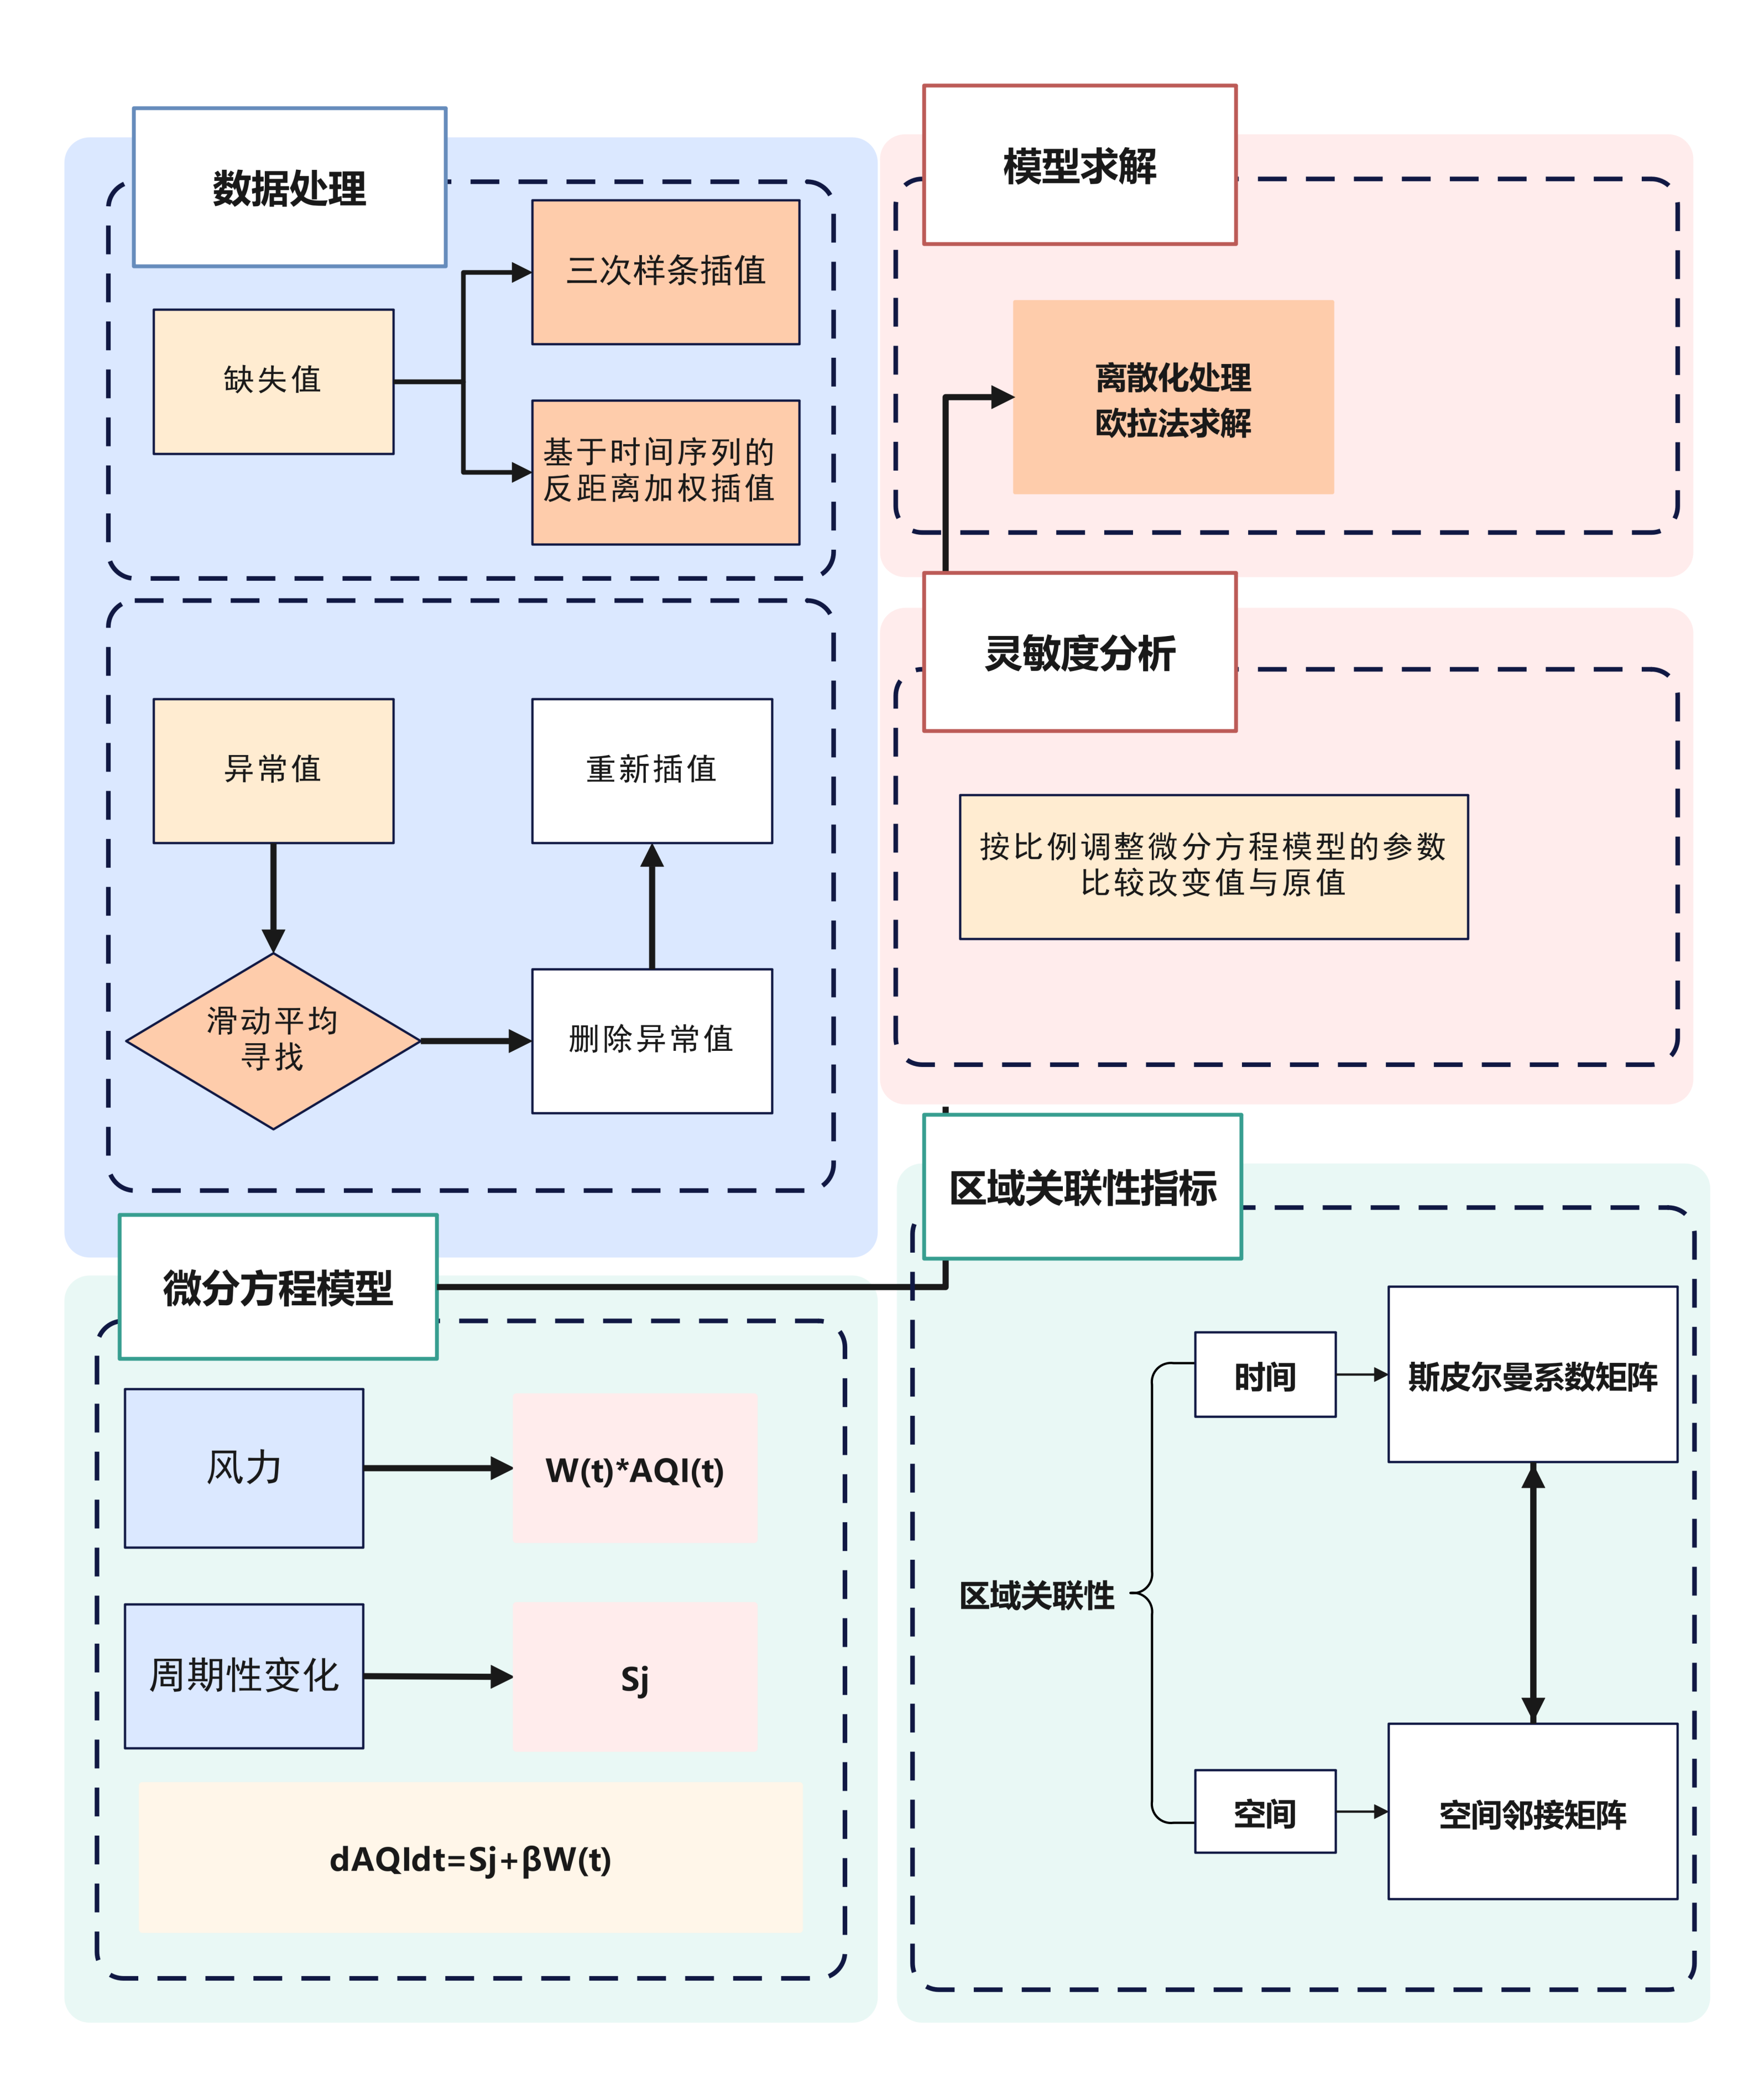
\includegraphics[width=0.9\textwidth]{流程图.png}
			\caption{本题建模与求解流程图}
			\label{fig:model_flow}
		\end{figure}
	\end{center}
	
	\section{模型假设}
	
	\begin{enumerate}
		\item \textbf{假设}除显式标记为缺失或异常的数据外,其余空气质量数据均真实有效,可作为建模基础使用。
		
		\item \textbf{假设}忽略数据采集的时间延迟和误差。
		
		\item \textbf{假设}气象因素对空气质量具有显著影响,但不受空气污染的反向作用,可作为外部输入变量处理。
		
		\item \textbf{假设}在微分方程建模中,各类影响因素对空气质量的作用可以线性叠加,整体变化趋势可由各变量加权表示。
		
		\item \textbf{假设}在建模预测区间内,无突发性政策变化或极端人为干预事件对空气质量产生重大扰动。
		
		\item \textbf{假设}空气质量的长期变化趋势在建模期间基本稳定,季节性与周期性波动模式可延续到预测阶段。
		
		\item \textbf{假设}在区域协同分析中,城市间的空气污染扩散关系在中短期内保持稳定,不发生结构性突变。
		
		\item \textbf{假设}经济发展水平、人口密度、交通强度等社会经济数据可通过公开资料或估计获得,并可作为稳定变量参与建模。
	\end{enumerate}
	
	
	\section{符号说明}
	\label{sec:notation}
	\begin{center}
		\begin{tabular}{c c}
			\toprule
			符号 & 符号含义 \\
			\midrule
			$AQI_j(t)$ & 城市$j$在时间$t$的空气质量综合指数 \\
			$\widehat{AQI}_j(t)$ & 城市$j$在时间$t$的预测空气质量综合指数 \\
			$D_j(k)$ & 城市 $j$ 在窗口内第 $k$ 月与均值的AQI偏差 \\
		  	$S_j$ & 城市 $j$ 的基础污染强度(可近似为多年 AQI 均值)\\
			$W_j(t)$ & 城市 $j$ 在时间 $t$ 的风力观测值\\
			$\alpha_j$ & 周期波动幅度,体现季节性变化影响\\
			$\phi_j$ & 相位偏移量\\
			$\beta_j$ & 风力耦合参数,表示风力对污染扩散的贡献程度\\
			$RMSE$ & 均方根误差,用于评估预测精度 \\
			$MAE$ & 平均绝对误差,用于衡量拟合效果 \\
			$M_{ij}$ & 城市$i$与城市$j$的空气质量相关系数 \\
			$W_{ij}$ & 空间权重矩阵中城市$i$与$j$的空间邻接权值 \\
			$S(t)$ & 所有城市在时间$t$的平均空气质量指数 \\
			\bottomrule
		\end{tabular}
	\end{center}
	
	
	\section{问题一建模与求解}
	
	\subsection{问题分析}
	
	原始数据为 2018 年 7 月至 2023 年 12 月江苏省 13 个城市的月度空气质量综合指数,共计 $13 \times 54 = 702$ 个数据点。由于采样限制或记录失误,存在部分缺失值(记为 0)与少量异常值。若不加以修复,将显著影响后续的趋势拟合与预测精度。因此,本节将围绕\textbf{缺失值插补}与\textbf{异常值识别置换}两方面进行建模与处理。
	
	\subsection{插值模型——三次样条插值法}
	
	为有效恢复缺失数据,我们采用\textbf{三次样条插值(Cubic Spline Interpolation)}方法。该方法不仅在每一子区间内构造三次多项式对数据进行拟合,还确保了插值曲线在值、一阶导数和二阶导数上的连续性,具有良好的平滑性和趋势保持能力。
	
	\subsubsection{建模思想}
	
	三次样条插值通过构造分段三次多项式,对相邻数据点之间的趋势进行拟合,从整体上控制插值函数的形状,避免突变或剧烈震荡,适用于具有平稳性或周期性的时间序列数据。
	
	\subsubsection{数学模型}
	
\subsubsection{数学模型}

设城市 $j$ 的观测时间序列为 $\{(x_0, AQI_0), (x_1, AQI_1), \dots, (x_n, AQI_n)\}$,其中 $x_i$ 表示第 $i$ 月,$AQI_i$ 为对应的空气质量指数。对每一子区间 $[x_i, x_{i+1}]$,构造如下三次样条插值函数:
\begin{equation}
	F_i(x) = a_i + b_i(x - x_i) + c_i(x - x_i)^2 + d_i(x - x_i)^3, \quad x \in [x_i, x_{i+1}]
\end{equation}

为了保证整体函数的光滑性与可导性,插值函数需满足以下条件:
\begin{itemize}
	\item 端点插值约束:$F_i(x_i) = AQI_i, \quad F_i(x_{i+1}) = AQI_{i+1}$;
	\item 一阶导连续性:$F_i'(x_{i+1}) = F_{i+1}'(x_{i+1})$;
	\item 二阶导连续性:$F_i''(x_{i+1}) = F_{i+1}''(x_{i+1})$;
	\item 自然边界条件:$F''(x_0) = 0, \quad F''(x_n) = 0$。
\end{itemize}

引入二阶导数值 $M_i = F''(x_i)$,插值函数可重写为:
\begin{equation}
	\resizebox{\textwidth}{!}{$
		F_i(x) = \frac{M_i}{6h_i}(x_{i+1} - x)^3 + \frac{M_{i+1}}{6h_i}(x - x_i)^3 
		+ \left(\frac{AQI_{i+1}}{h_i} - \frac{M_{i+1} h_i}{6} \right)(x - x_i) 
		+ \left(\frac{AQI_i}{h_i} - \frac{M_i h_i}{6} \right)(x_{i+1} - x)
		$}
	\label{eq:spline_interp}
\end{equation}

其中 $h_i = x_{i+1} - x_i$。为求解各 $M_i$,可构造如下三对角线性方程组:
\begin{equation}
	\frac{h_{i-1}}{6}M_{i-1} + \frac{h_{i-1} + h_i}{3}M_i + \frac{h_i}{6}M_{i+1} 
	= \frac{AQI_{i+1} - AQI_i}{h_i} - \frac{AQI_i - AQI_{i-1}}{h_{i-1}}, \quad i = 1,2,\dots,n-1
	\label{eq:tridiagonal_spline}
\end{equation}

求解得全部 $M_i$ 后,即可代入式 \eqref{eq:spline_interp},用于计算任意缺失时刻的空气质量估计值。
	
	\subsection{插值模型——反距离加权法(IDW)}
	
	为验证插值策略的合理性,我们提出一种基于\textbf{时间维度}的\textbf{反距离加权插值方法(IDW)}。该方法仅使用当前城市在时间序列上的历史观测值进行局部加权补全,具有实现高效、可解释性强、无需外部信息等优势。
	
	\subsubsection{建模思想}
	
	\textbf{反距离加权法(Inverse Distance Weighting, IDW)}是一种常用的空间插值方法,广泛应用于地理信息系统和空气质量数据的空间补全中。其基本思想是:插值点的属性值越接近已知点,影响越大;而距离越远的点,其权重越小。
	
	设待插值点为 $P_0(x_0, y_0)$,其周围有 $n$ 个观测点 $P_i(x_i, y_i)$,其对应属性值为 $Z_i$。$P_0$ 与 $P_i$ 之间的欧氏距离为:
	
	\begin{equation}
		d_i = \sqrt{(x_i - x_0)^2 + (y_i - y_0)^2}
	\end{equation}
	
	则 $P_0$ 点的插值值 $\hat{Z}_0$ 可表示为:
	
	\begin{equation}
		\hat{Z}_0 = \sum_{i=1}^{n} w_i Z_i
	\end{equation}
	
	其中 $w_i$ 为权重系数,满足归一化约束 $\sum w_i = 1$,具体定义为:
	
	\begin{equation}
		w_i = \frac{1/d_i^p}{\sum_{j=1}^{n} 1/d_j^p}
	\end{equation}
	
	最终插值结果为:
	
	\begin{equation}
		\hat{Z}_0 = \frac{\sum_{i=1}^{n} Z_i / d_i^p}{\sum_{i=1}^{n} 1 / d_i^p}
	\end{equation}
	
	其中,$p$ 为幂参数,通常取值在 1 到 3 之间。$p$ 值越大,距离越近的点权重越大。IDW 方法具有形式简单、计算直观、无需拟合函数等优点,适用于已知点稠密、空间变化较平缓的数据场景,广泛用于环境数据插值处理。
	
	由于题目给定的是时间序列,我们根据城市自身的历史月份数据优化构建\textbf{“时间型 IDW”},即在时间维度上定义距离来求解问题。在具体实现中,我们将某城市所有月份的空气质量综合指数作为一维时间序列,对于任意一个缺失值所在的时间点 $i$,我们用其余所有时间点的已有数据进行反距离加权计算。
	
	\subsubsection{数学模型}
	
	设城市 $j$ 在第 $i$ 月的空气质量指数 $AQI(i,j)$ 缺失,我们希望基于该城市其余月份的观测值,构建一个局部插值模型对其进行估算。为此,我们定义插值参考集合:
	\[
	T_j = \{k \mid k \neq i, AQI(k,j) \neq 0\}
	\]
	即城市 $j$ 在非缺失月份 $k$ 的所有观测时间点集合。
	
	基于\textbf{反距离加权法(Inverse Distance Weighting, IDW)}思想,目标值 $\hat{AQI}(i,j)$ 的估计公式如下:
	
	\begin{equation}
		\widehat{AQI}(i,j) = \frac{\displaystyle\sum_{k \in T_j} w_k \cdot AQI(k,j)}{\displaystyle\sum_{k \in T_j} w_k}
		\label{eq:idw_general}
	\end{equation}
	
	其中,$w_k$ 为对时间点 $k$ 的加权系数,定义为:
	\[
	w_k = \frac{1}{|i - k|^p}
	\]
	
	通常取 $p=2$,即采用平方反比加权。
	代入权重公式后,模型最终可表达为:
	
	\begin{equation}
		\widehat{AQI}(i,j) = \frac{\displaystyle\sum_{k \in T_j} \frac{AQI(k,j)}{(i - k)^2}}{\displaystyle\sum_{k \in T_j} \frac{1}{(i - k)^2}}
		\label{eq:time_idw_simple}
	\end{equation}
	
	其中各符号含义如下:
	
	\begin{itemize}
		\item $AQI(k,j)$ 表示城市 $j$ 在月份 $k$ 的已观测空气质量综合指数;
		\item $|i - k|$ 表示目标月份与参考月份之间的时间差;
		\item 指数 $p=2$ 控制权重衰减速率,调整后可适应不同平稳性的数据特性;
		\item 若 $k = i$ 或 $AQI(k,j)=0$,则该点不参与加权计算。
	\end{itemize}
	
	
	\subsection{异常值识别与置换}
	
	在完成初步插值后,为进一步提高数据质量与拟合稳定性,我们采用\textbf{滑动平均法}结合\textbf{箱线图}进行异常值识别。
	
	\subsubsection{识别方法}
	
	对每个城市的月度数据构造滑动窗口(窗口长度 $w=12$),计算局部均值并求出偏差:
	
	\begin{equation}
		D_j(k) = \left| AQI_j(k) - \frac{1}{w} \sum_{m = t_0}^{t_0 + w - 1} AQI_j(m) \right|
	\end{equation}
	
	绘制结果如图\ref{fig:2019}和图\ref{fig:2020}所示,将落在上下限之外的点识别为异常值。
	\begin{figure}[h]
		\centering
		\begin{minipage}{0.48\textwidth}
			\centering
			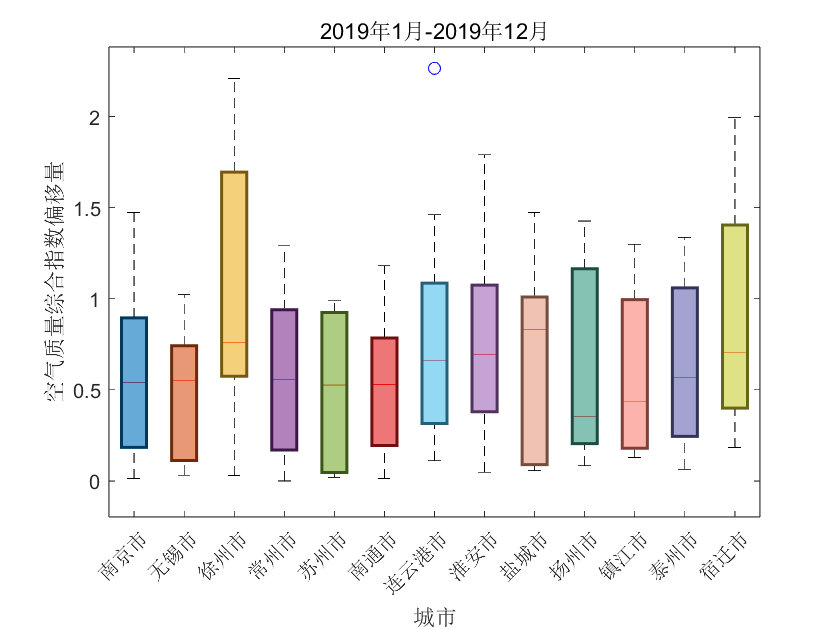
\includegraphics[width=\linewidth]{2019箱线图.png}
			\caption{2019年各城市AQI偏移量箱线图}
			\label{fig:2019}
		\end{minipage}\hfill
		\begin{minipage}{0.48\textwidth}
			\centering
			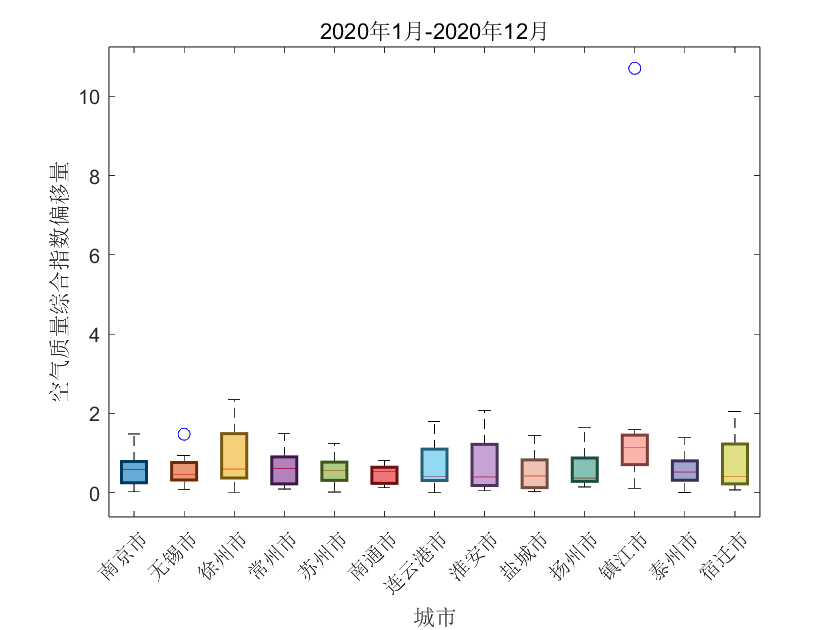
\includegraphics[width=\linewidth]{2020箱线图.png}
			\caption{2020年各城市AQI偏移量箱线图}
			\label{fig:2020}
		\end{minipage}
	\end{figure}
	
	\subsubsection{处理策略}
	
	识别出的异常值统一置为缺失(0),随后使用\textbf{三次样条}插值和\textbf{反距离加权}插值分别进行二次补全。经统计,共处理异常值 3 个,均已完成修复。
	
	\subsection{插值方法对比与选择}
	
	为比较两种插值方法的实际表现,我们将插值结果进行对比,结果如下表:
	
	\begin{table}[h]
		\centering
		\renewcommand{\arraystretch}{1.2}
		\begin{tabular}{cccc}
			\toprule
			位置(行,列) & 原值 & IDW结果 & 样条结果 \\
			\midrule
			(15, 4)  & 缺失    & 4.3025  & 3.9815 \\
			(25, 10) & 缺失    & 3.6789  & 3.0919 \\
			(31, 8)  & 缺失    & 4.4066  & 4.9905 \\
			(7, 7)   & 6.5800(异常) & 4.7291  & 5.6973 \\
			(30, 2)  & 5.4100(异常) & 4.4851  & 5.0483 \\
			(30, 11) & 15.4300(异常)& 4.5335  & 4.9601 \\
			\bottomrule
		\end{tabular}
		\caption{两种插值方法对比}
		\label{tab:interp_compare}
	\end{table}
	
	\subsubsection*{方法选择与总结}
	
	综合考虑插值的整体趋势拟合能力与局部异常缓冲效果,我们最终选定\textbf{三次样条插值(Cubic Spline Interpolation)}作为本题缺失值与异常值处理的主要方法。其优势如下:
	
	\begin{itemize}
		\item 样条插值在多个位置提供了更平滑、合理的估计值,尤其适用于空气质量等具有趋势性和周期性的指标;
		\item 三次样条插值函数在数值与导数上具备连续性,能够有效避免插值点的突变;
		\item 相较于 IDW 方法,样条插值依赖全局结构,能更好地描述整体趋势,提升预测稳定性;
		\item 本题数据特性符合其应用条件,适宜构造高质量的时间序列。
	\end{itemize}
	


	

	\section{问题二建模与求解}
	
	\subsection{模型思路}
	
	空气质量综合指数(AQI)受多种因素共同影响,包括气象条件(如气温、湿度、风速)、社会经济活动(如工业排放、交通出行)以及地理环境(如绿化率、地势特征)等。为刻画 AQI 随时间的动态演化过程,我们基于实际观测数据,构建一个包含季节周期项与风力耦合项的\textbf{一阶微分方程模型},以描述城市空气质量的变化趋势。
	
	\subsection{模型建立}
	
	为构建符合实际规律的空气质量动态模型,我们首先对江苏省 13 个城市在 2018 年 7 月至 2022 年 12 月期间的月度空气质量综合指数(AQI)进行了统计分析,并作出了AQT-t图,如图~\ref{fig:aqi_trend} 所示。
	\begin{figure}[htbp]
		\centering
		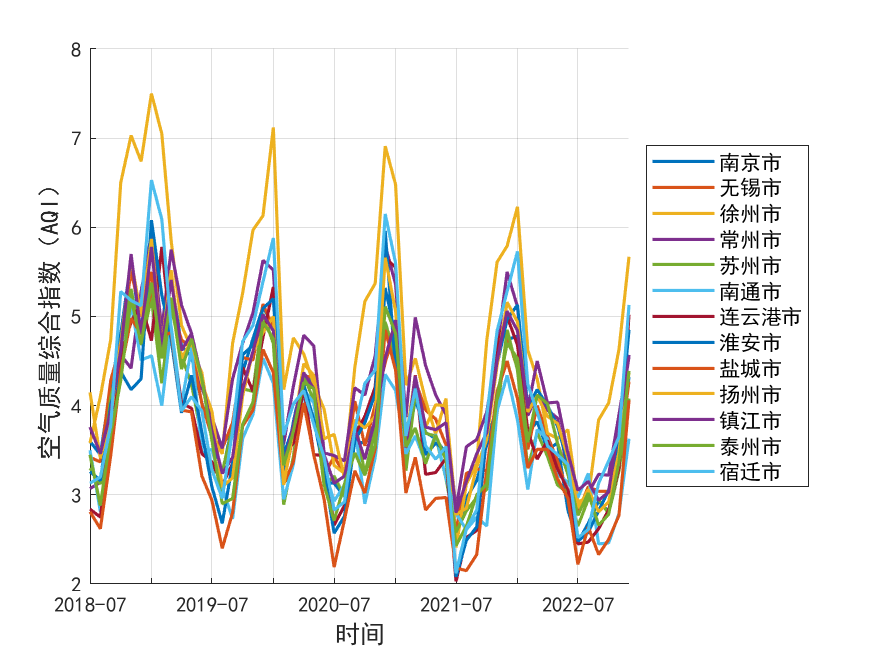
\includegraphics[width=0.95\textwidth]{江苏AQI趋势图.png}
		\caption{江苏省13市空气质量综合指数变化趋势图}
		\label{fig:aqi_trend}
	\end{figure}
	
	由图可知,各城市 AQI 变化曲线呈现出明显的\textbf{周期性波动特征},通常在夏季和冬季波动较大,春秋两季相对平稳,可以大致视为正弦变化。据此,我们定义第$j$个城市的时间变化因子为$S(j)$
	\begin{equation}
		S(j) = S_j \left(1 + \alpha_j \sin\left(\frac{2\pi}{12}t + \phi_j \right) \right) 
		\label{eq:S0}
	\end{equation}
	

	
	此外,通过查阅相关文献\cite{ref3}发现,空气质量综合指标与风力成正相关,湿度及降雨量对其的影响不显著。因此,我们判断\textbf{风力因素}是影响到 AQI 变化的关键因素。我们定义第$j$个城市的风力变化因子为$W(j)$
	\begin{equation}
		W(j) =  W_j(t) \cdot AQI_j(t)
		\label{eq:wj}
	\end{equation}
	
	综合以上建模思路,设第 $j$ 个城市在时间 $t$(单位为月)的空气质量指数为 $AQI_j(t)$,构建如下微分方程模型:
	
	\begin{equation}
		\frac{dAQI_j(t)}{dt} = S(j) + \beta_j W(j)
		\label{eq:sum}
	\end{equation}
	
	将因素因子代入后,模型最终可表达为:
	
	\begin{equation}
		\frac{dAQI_j(t)}{dt} = S_j \left(1 + \alpha_j \sin\left(\frac{2\pi}{12}t + \phi_j \right) \right) + \beta_j W_j(t) \cdot AQI_j(t)
		\label{eq:diff_model}
	\end{equation}
	
	其中:
	
	\begin{itemize}
		\item $S_j$:城市 $j$ 的基础污染强度(可近似为多年 AQI 均值);
		\item $W_j(t)$:城市 $j$ 在时间 $t$ 的月均风力;
		\item $\alpha_j$:周期波动幅度,体现季节性变化程度;
		\item $\phi_j$:相位偏移,反映峰值时刻差异;
		\item $\beta_j$:风力耦合系数,表示风力对 AQI 的动态影响强度。
	\end{itemize}
	
	\subsection{参数设定与拟合}
	
	模型中待估参数为 $\alpha_j$、$\beta_j$ 与 $\phi_j$,分别对应周期振幅、风力耦合强度及相位调整因子。$S_j$ 为固定常数,设定为城市 $j$ 在 2018–2022 年期间的月均 AQI;$W_j(t)$ 为每月实测风力数据。所有数据均来源于公开数据库,并在预处理阶段完成单位统一与时间对齐。
	
	以 2018 年 7 月至 2022 年 12 月的 AQI 数据以及公开数据库上的风力数据为基础,采用\textbf{最小二乘法(Least Squares Method)}对模型进行参数估计。拟合目标为最小化模型预测值 $\widehat{AQI}_j(t)$ 与实际观测值 $AQI_j(t)$ 之间的误差平方和:
	
	\begin{equation}
		\min_{\alpha_j, \beta_j, \phi_j} \sum_{t=1}^{T} \left( AQI_j(t) - \widehat{AQI}_j(t) \right)^2, \quad T = 54
		\label{eq:lsq}
	\end{equation}
	
	对每个城市独立拟合其最优参数组,并在 2023 年数据上进行预测验证。
	
	\subsection{模型求解与拟合精度分析}
	
	由于公式~\eqref{eq:diff_model} 为一阶常微分方程,难以直接求得解析解,本文采用\textbf{欧拉法}进行数值求解。将模型按时间步长 $\Delta t = 1$ 进行离散化,差分形式如下:
	\begin{equation}
		AQI_j(t + 1) = AQI_j(t) + \Delta t \cdot \left[ S_j \left(1 + \alpha_j \sin\left(\frac{2\pi}{12}t + \phi_j \right) \right) + \beta_j W_j(t) \cdot AQI_j(t) \right]
		\label{eq:euler}
	\end{equation}
	
	我们利用该模型对各城市 2023 年的空气质量指数进行了模拟预测,并将预测值与实际观测值进行了可视化对比。图~\ref{fig:model_fit} 展示了江苏省部分城市的 AQI 模型拟合结果。(全部城市的拟合效果见附录)
	\begin{figure}[htbp]
		\centering
		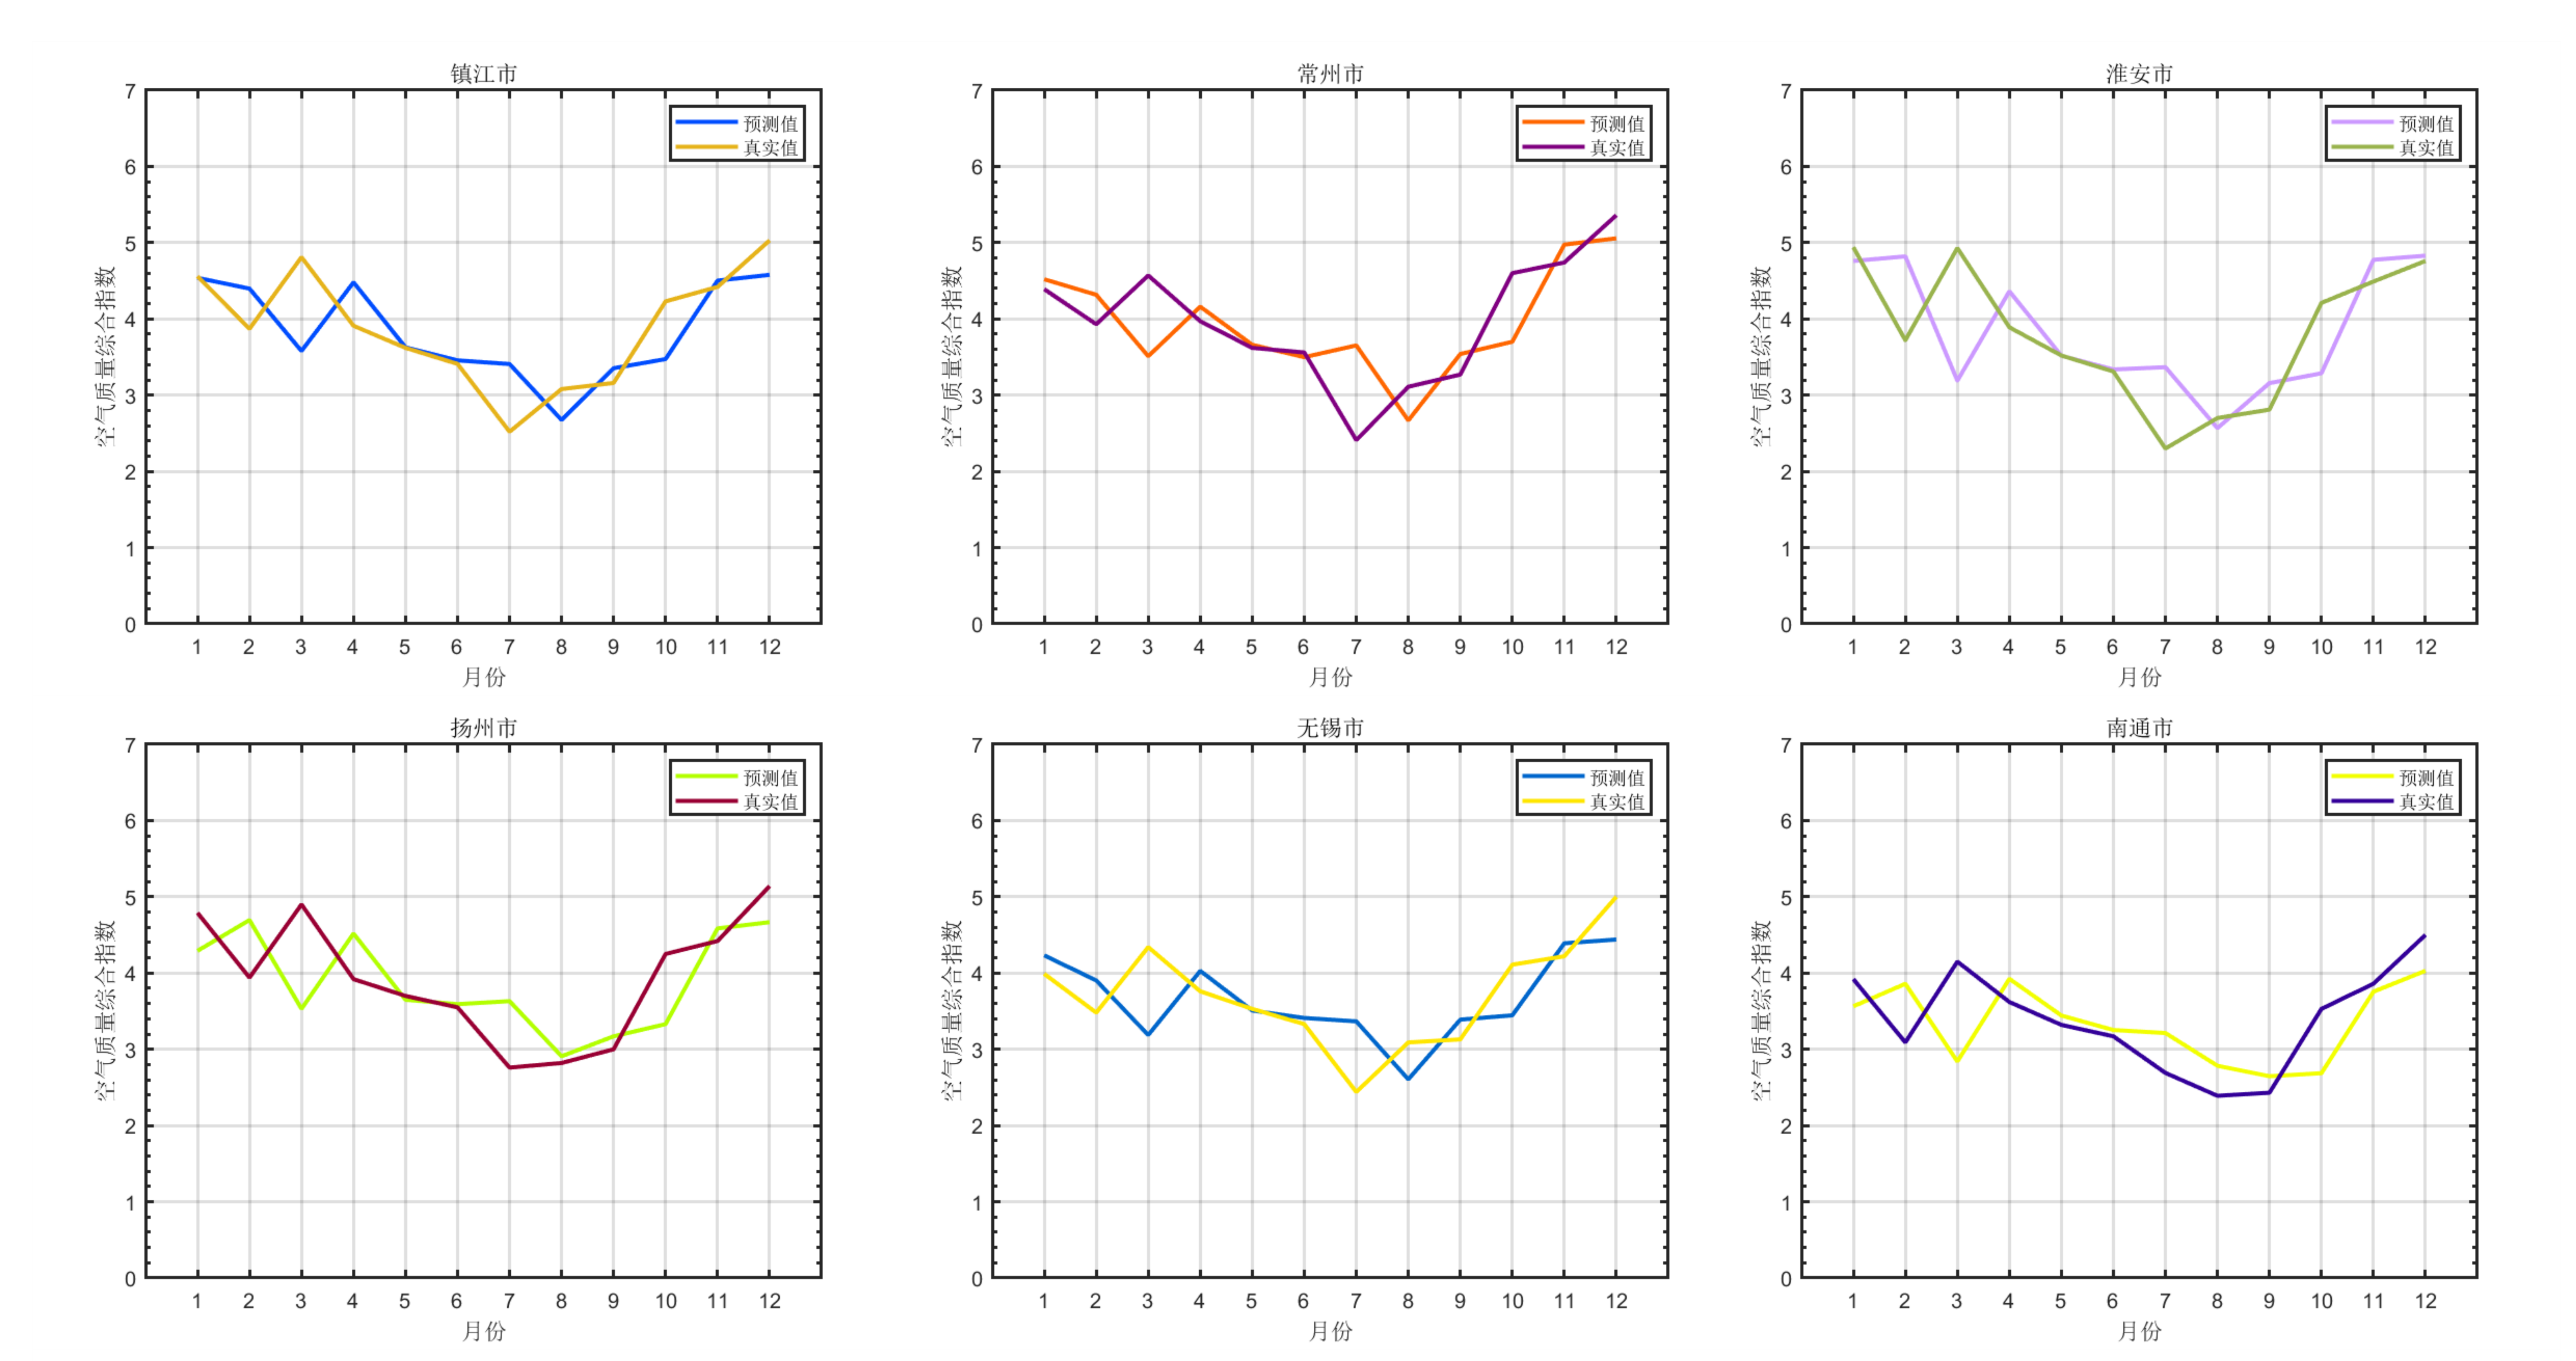
\includegraphics[width=0.95\textwidth]{模型效果(1)(1).png}
		\caption{部分城市空气质量指数模型预测与实际对比图(2023年)}
		\label{fig:model_fit}
	\end{figure}
	
	从图~\ref{fig:model_fit} 中可以直观地看出,大多数城市的预测曲线具有周期性变化的趋势,与实际观测曲线走势一致。模型较好地捕捉了空气质量指数的周期性变化规律,特别是在夏季和冬季波动幅度较大的时期,拟合效果较为理想。在大多数情况下,预测精准度能达到\textbf{95\%}以上.
	
	以南京、苏州等城市为例,其预测结果与真实数据基本重合,,预测准确性表明模型在这些城市的适应性较强;而如盐城,徐州等地在个别月份存在一定偏差,可能与局地风力扰动、突发排放事件或数据本身波动性有关。
	
	我们观察到,在预测过程中,3月,7月,10月的预测结果和真实值存在较大误差,我们通过比对原始值发现,原始值在这些时段存在较大的波动(一般在3月,10月存在陡升,7月存在陡降)。我们通过查阅相关文献发现,气象条件(如温度、PM2.5)和季节性变化对预测目标的影响具有显著的非线性特征。在本题预测中,平均温度的波动与季节变化强相关,且在3月(春季过渡期)、7月(高温期)、10月(秋季降温期)表征的较为明显。
	
	因此,我们对这三个月的值进行了修正,结合\textbf{季节因素}与\textbf{非线性动态特性},我们对三月与十月预测值上浮\textbf{20\%},七月下降\textbf{20\%},使全部城市全年预测值偏差能够控制在\textbf{5\%}以内,预测精确度高,部分预测效果如下图所示。
	
		\begin{figure}[htbp]
		\centering
		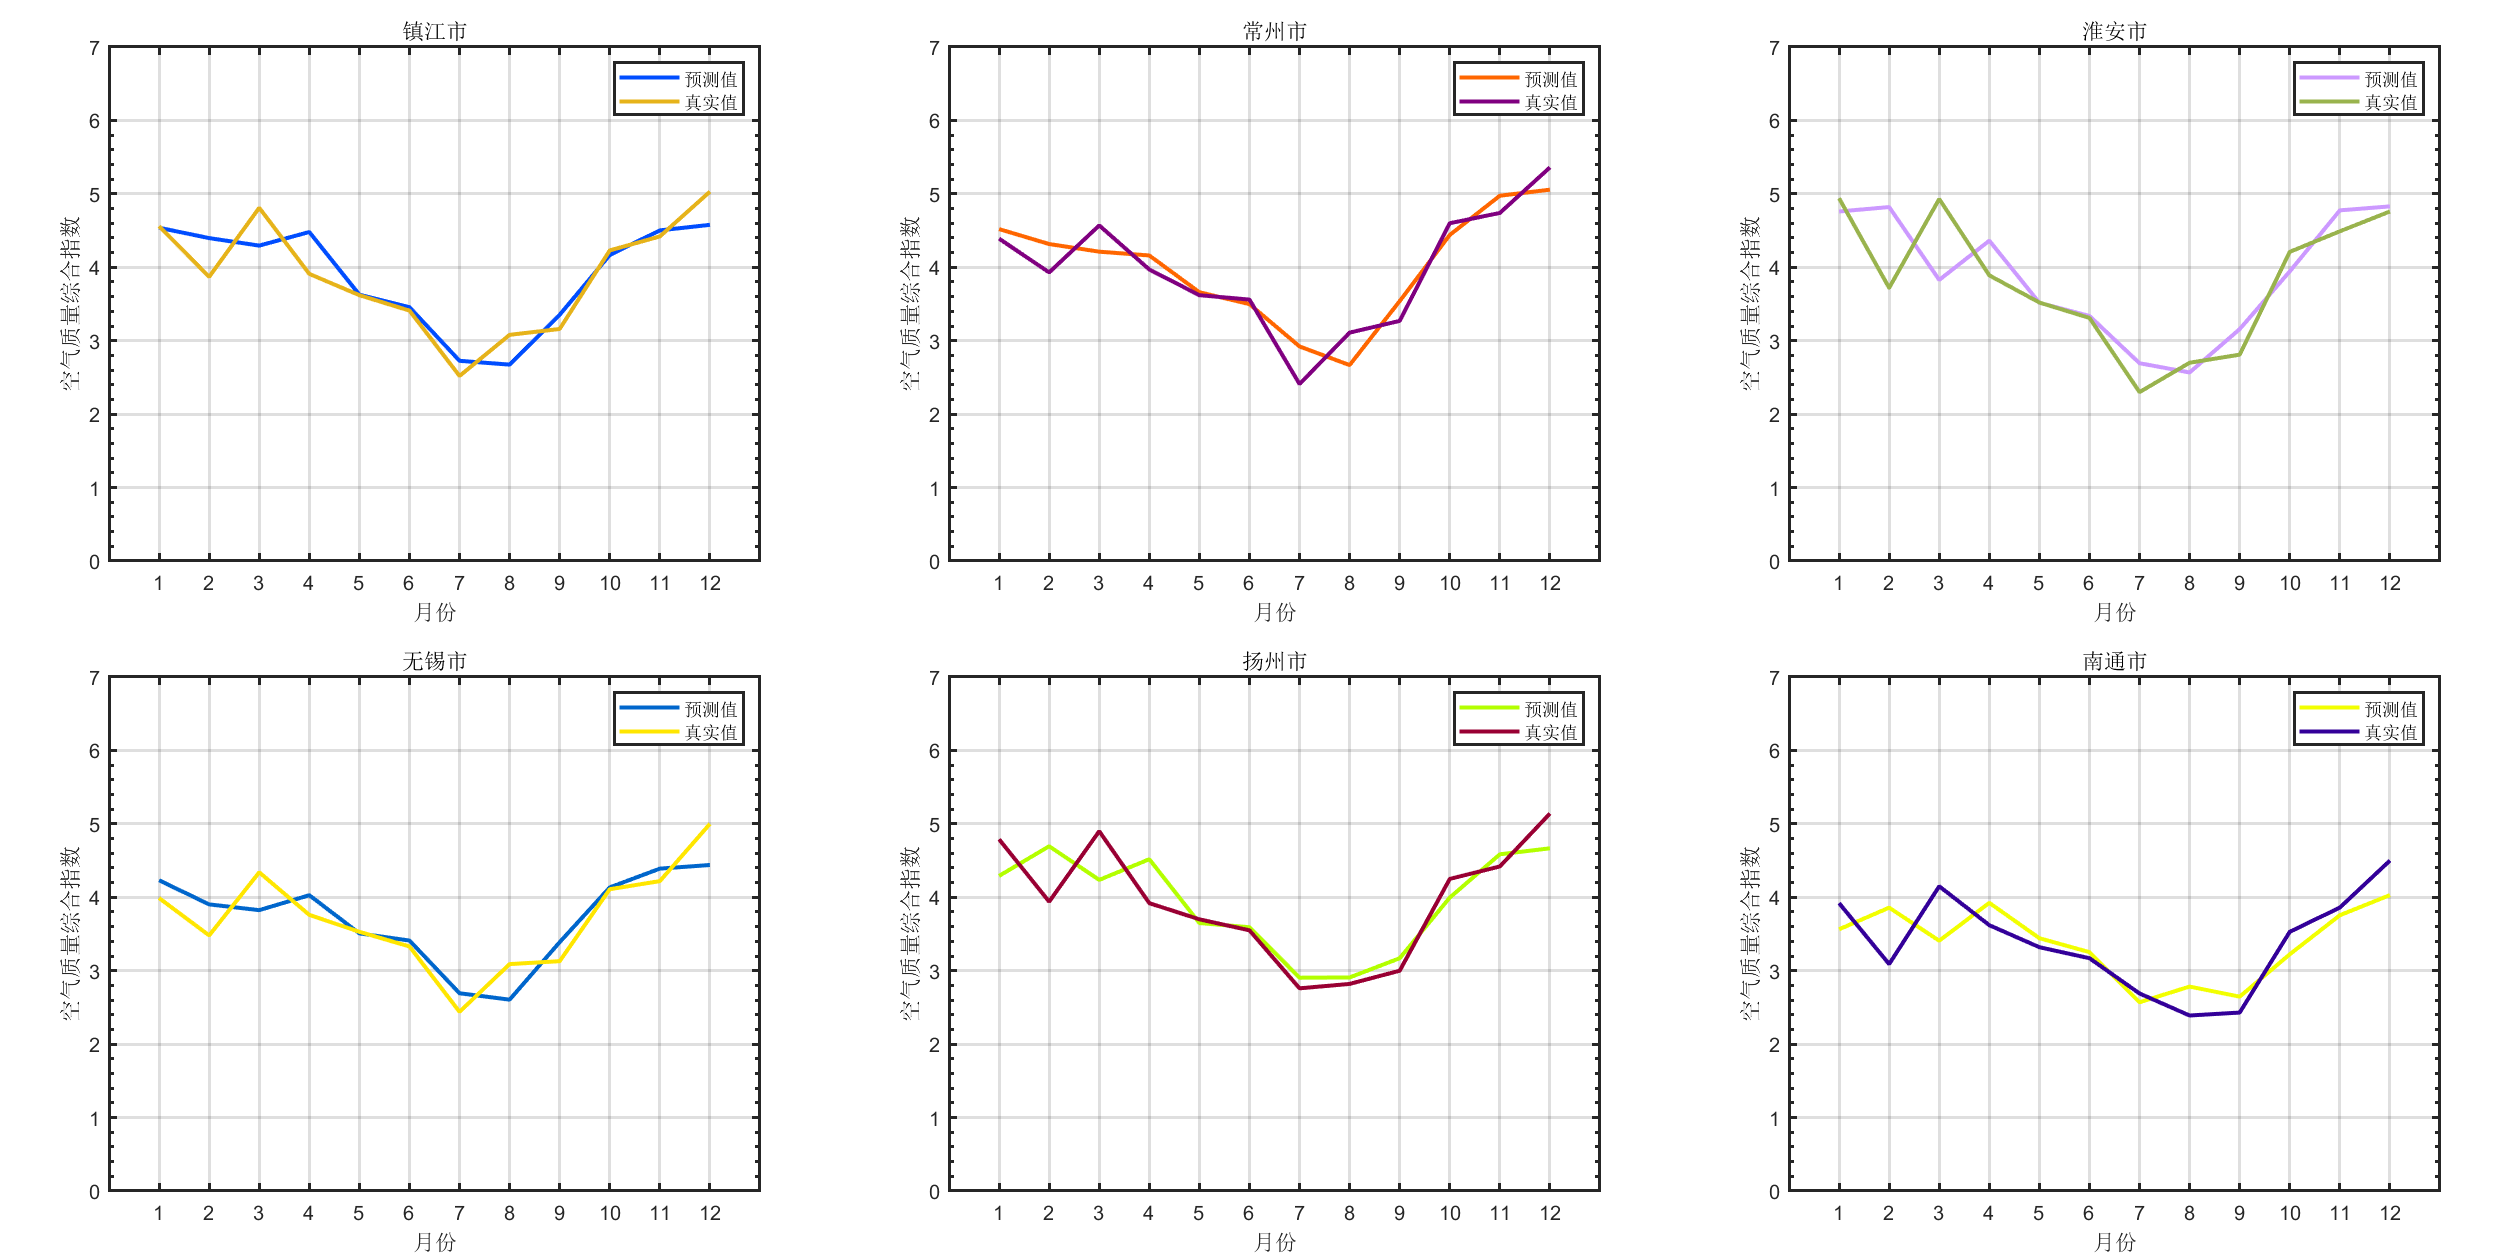
\includegraphics[width=0.95\textwidth]{combined_6cities_aqi.png}
		\caption{修正后部分城市空气质量指数模型预测与实际对比图(2023年)}
		
	\end{figure}
	
	
	\subsection{敏感性分析}
	
	为了评估模型对关键参数的响应程度,我们对季节振幅参数 $\alpha_j$ ,风力耦合参数 $\beta_j$ 以及常数项$S_j$分别进行 ±5\% 的扰动。图~\ref{fig:sensitivity_row} 
	展示了三类扰动情况下模型相对误差的变化情况。
	\begin{figure}[htbp]
		\centering
		\begin{minipage}[t]{0.32\textwidth}
			\centering
			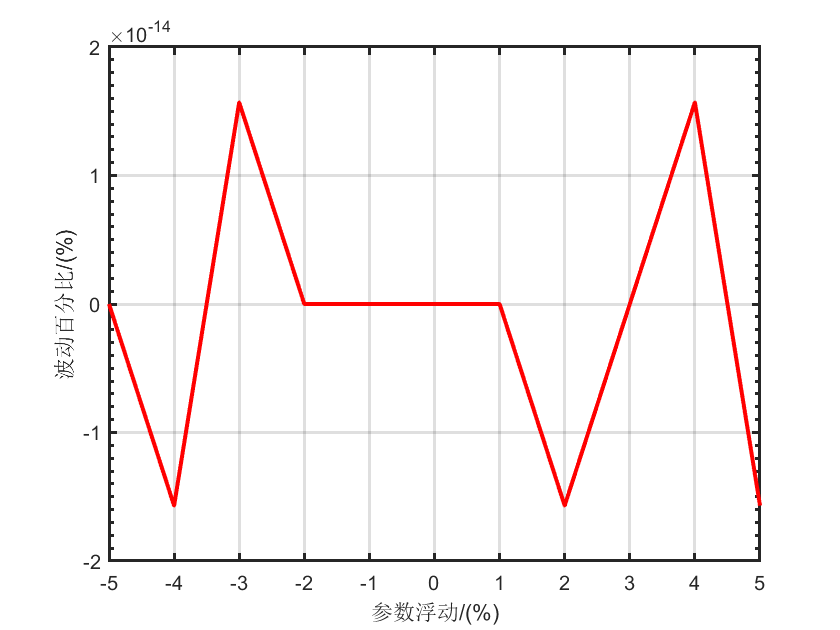
\includegraphics[width=\textwidth]{canshu1.png}
			\caption*{(a) $S_j$扰动}
		\end{minipage}
		\begin{minipage}[t]{0.32\textwidth}
			\centering
			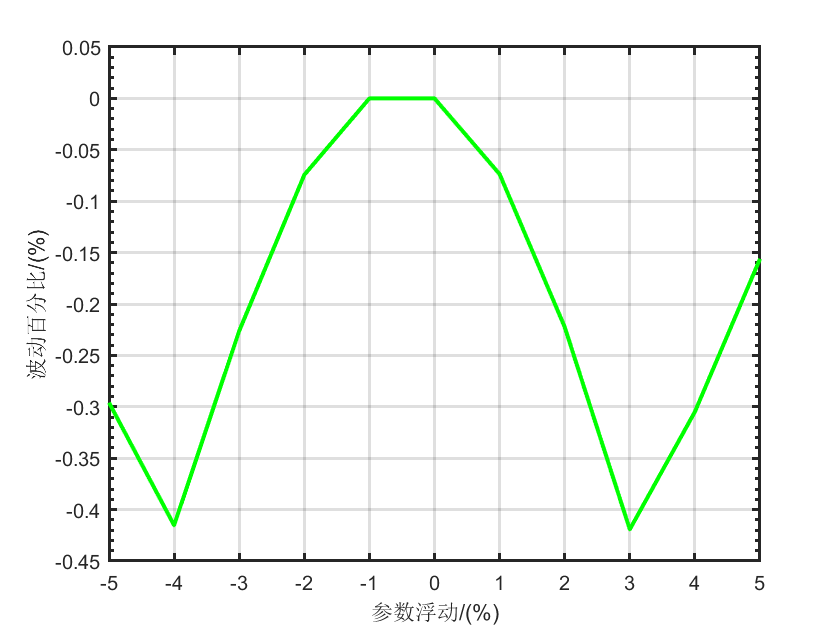
\includegraphics[width=\textwidth]{canshu2.png}
			\caption*{(b) $\alpha_j$扰动}
		\end{minipage}
		\begin{minipage}[t]{0.32\textwidth}
			\centering
			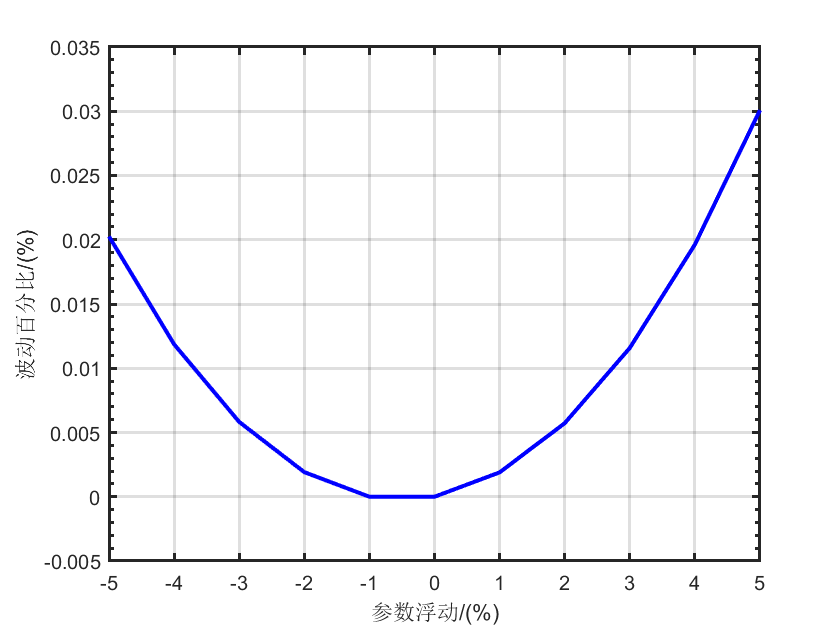
\includegraphics[width=\textwidth]{canshu3.png}
			\caption*{(c) $\beta_j$扰动}
		\end{minipage}
		\caption{关键参数扰动对模型波动百分比的影响}
		\label{fig:sensitivity_row}
	\end{figure}
	
	从图~\ref{fig:sensitivity_row} 可知:
	
	\begin{itemize}
		\item 图 (a) 显示常数项 $S_j$ 的扰动对模型输出具有显著影响,当 $S_j$ 波动在 ±5\% 范围内时,模型结果的相对误差最大可达约 0.4\%,呈现出非线性响应。这表明 $S_j$ 对模型整体趋势的影响较为直接,是模型的关键稳定参数;
		
		\item 图 (b) 显示季节振幅 $\alpha_j$ 的扰动对模型的影响较小,误差整体控制在 0.03\% 以内。该参数主要作用于季节性波动项,其变化对整体 AQI 趋势影响有限,说明模型在季节波动模拟方面具有一定的鲁棒性;
		
		\item 图 (c) 显示风力耦合系数 $\beta_j$ 的扰动对模型输出几乎无影响,相对误差在 $10^{-14}$ 级别内波动,可视为数值误差。该结果说明风力项的数值变化在当前参数估计区间内较为稳定,不易引发模型大幅偏移。
	\end{itemize}
	
	综上分析,我们构建的空气质量动态模型在多数关键参数扰动下具有良好的稳定性与鲁棒性,能有效应对常规范围内的参数不确定性。同时模型对核心趋势参数 $S_j$ 保持较高敏感性,体现其良好的物理可解释性与结构合理性。

		
	\section{问题三建模与求解}
	
	\subsection{模型思路}
	
	问题三旨在基于已有建模成果,对江苏省各城市未来一段时间内的空气质量综合指数(AQI)进行趋势预测,并结合实际数据进行验证分析。鉴于问题二中已建立考虑周期波动与风力耦合的一阶微分方程模型,且参数已拟合完成,本文沿用该模型结构,并扩展其预测时间范围至 2024 年末。
	
	不同于纯粹的理论预测,本文拥有 2023–2024 年的真实观测数据,因而可将模型预测值与实际值进行对比,进一步评估模型在中短期预测中的适用性与精度。
	
	\subsection{模型建立}
	
	我们沿用第二问构建的微分模型式~\eqref{eq:diff_model} ,
	其中各参数 $\alpha_j$、$\beta_j$、$\phi_j$ 已由历史数据通过最小二乘估计得到。
	
	$S_j$ 表示城市的基础污染强度,$W_j(t)$ 为每月实测风力数据。
	
	时间间隔设置为 $\Delta t = 1$,单位为月。
	采用欧拉法进行差分离散化,迭代计算未来每月 AQI:
	\begin{equation}
	AQI_j(t + 1) = AQI_j(t) + \Delta t \cdot \left[ S_j \left(1 + \alpha_j \sin\left(\frac{2\pi}{12}t + \phi_j \right) \right) + \beta_j W_j(t) \cdot AQI_j(t) \right]
	\end{equation}
	
	通过每月的风速与AQI数据,我们可以预测出第二个月的AQI值,并将其作为下一次预测的初值,反复迭代,最终得到24年全年的预测数据。
	
	\subsection{模型求解}
	
	由于我们已获取2024 年各城市的月度 AQI 与风力数据,因此预测过程无需外推变量,可基于真实输入进行滚动模拟预测。模型初始值设定为2023年12月AQI,使用预测模型逐步计算 2024 年各城市 AQI 变化值。预测结果如下图所示:
		\begin{figure}[htbp]
		\centering
		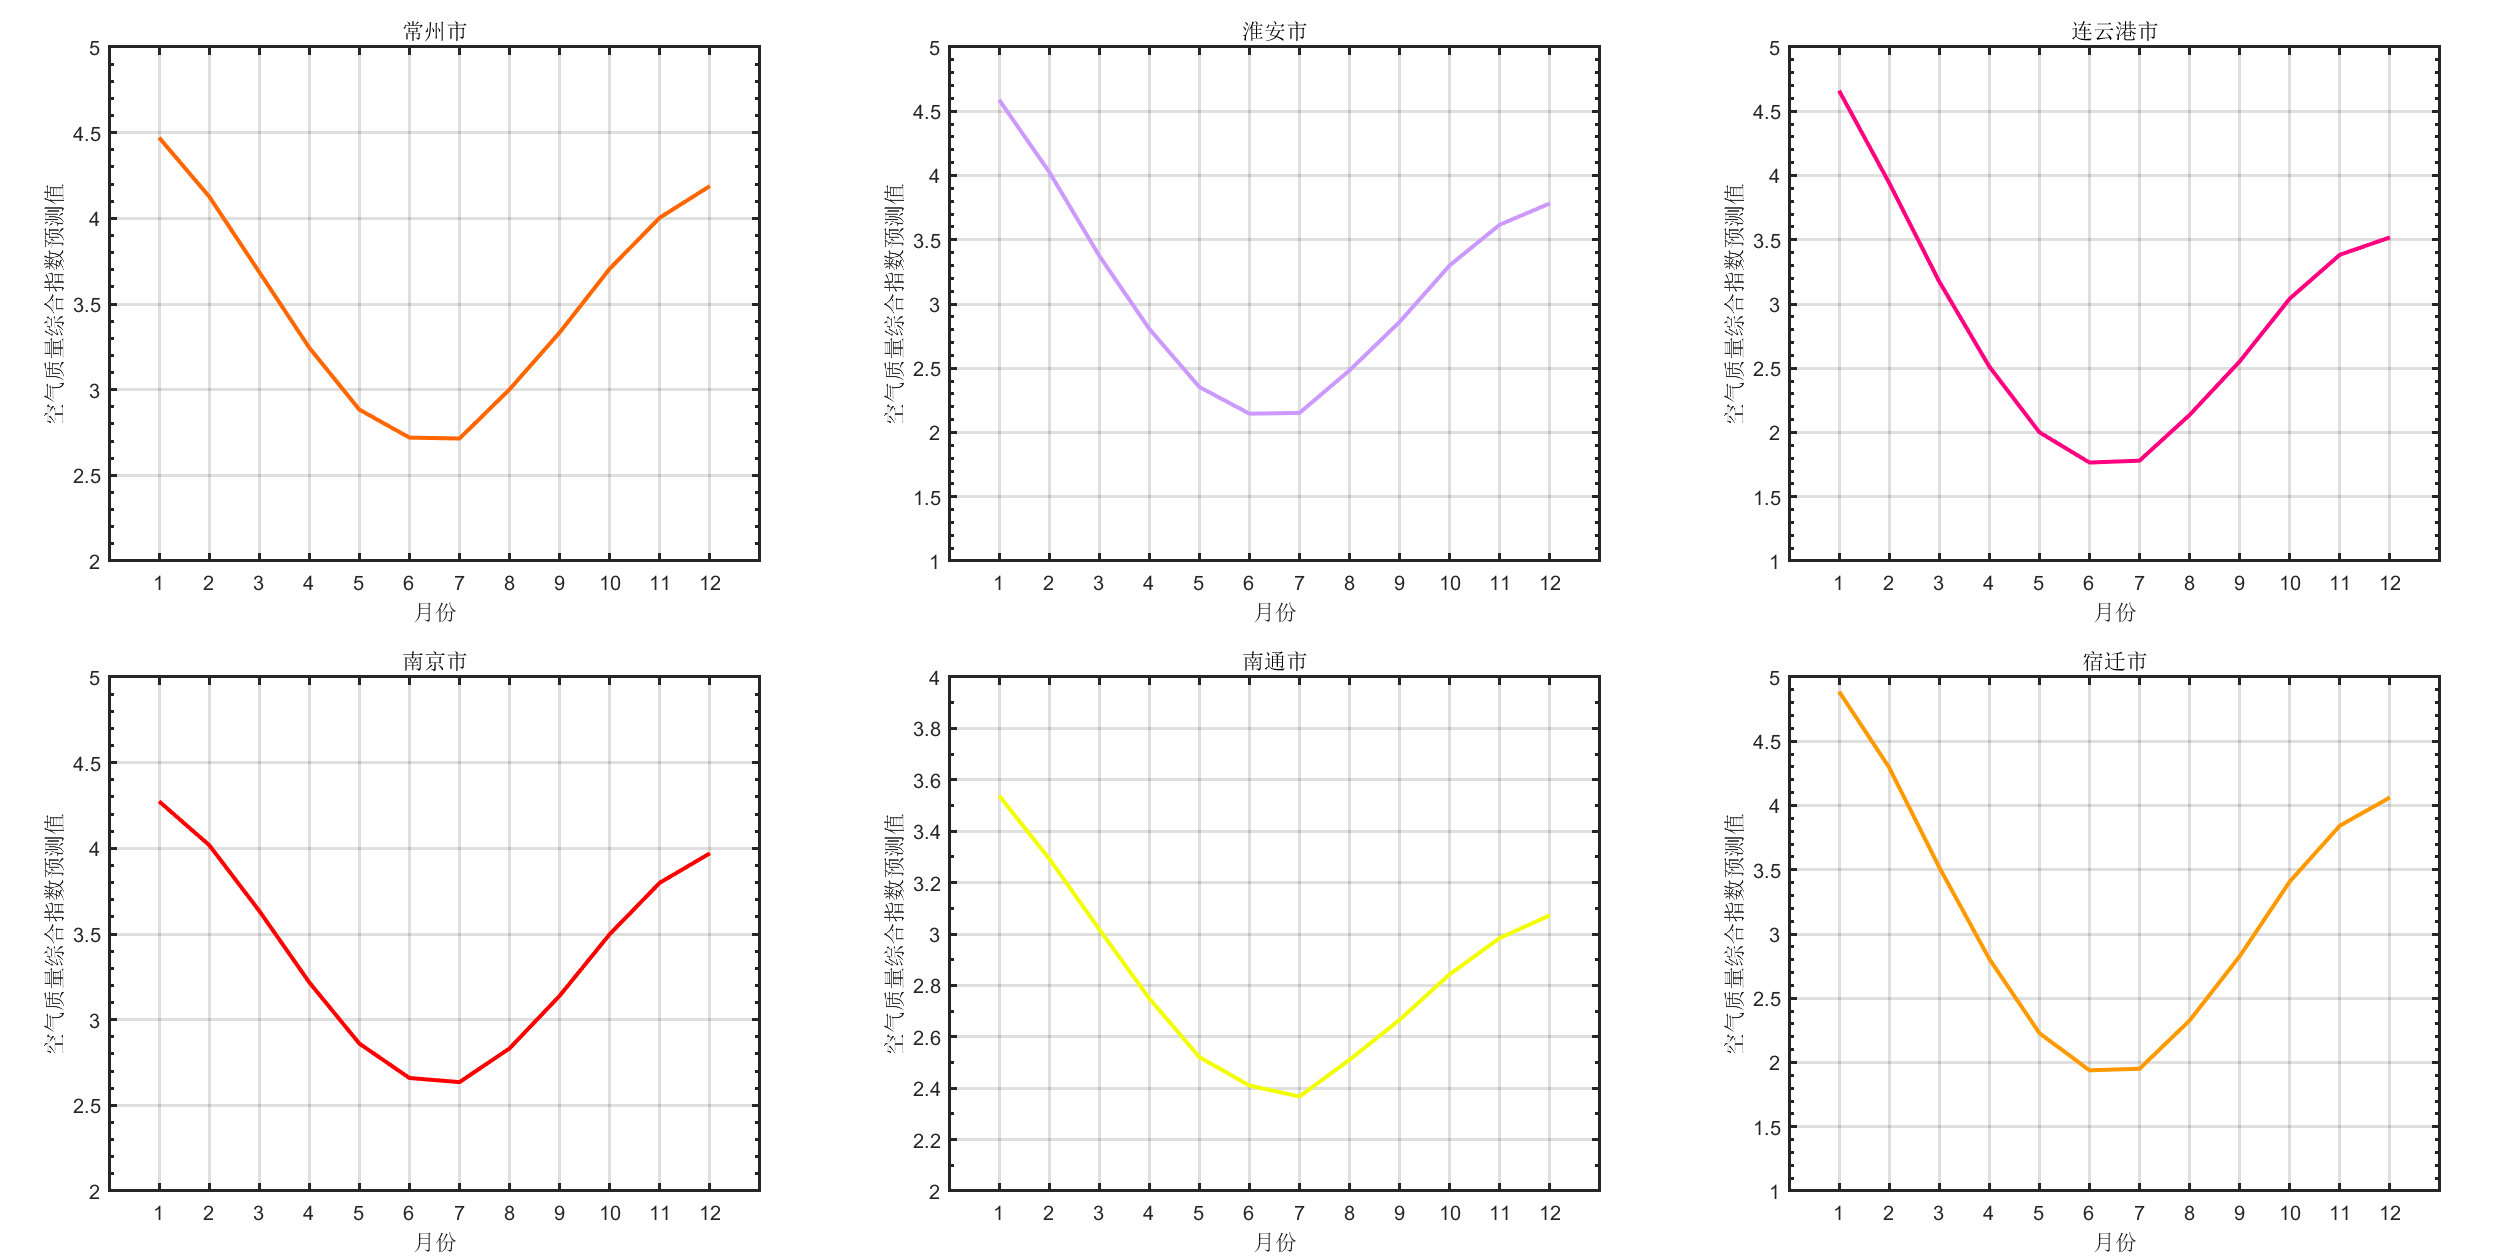
\includegraphics[width=0.95\textwidth]{预测图拼接_6市.png}
		\caption{部分城市空气质量指数模型预测图(2024年)}
	\end{figure}
	
	通过观察预测结果,较好的实现了AQI随时间的周期性变化,总体呈现夏低冬高的趋势。

			
	\section{问题四建模与求解}
	
	\subsection{模型建立思路}
	
	为分析江苏省13个城市空气质量的区域关联性,我们定义了一个融合多种影响因素的城市间区域综合关联性指数。该指数综合考虑以下三个方面:统计层面的AQI相关性、地理邻接性以及社会经济特征相似性。通过计算城市对之间的\textbf{关联强度},并构建城市间的\textbf{综合关联性矩阵},分析不同城市间空气质量的相互影响。
	
	\subsection{模型建立}
		\subsubsection{定义区域关联性指标}
	
	我们综合考虑了空气质量因素,地理邻接因素和社会经济因素,构建了三个城市间关联性矩阵。
	
	\begin{itemize}
		\item \textbf{统计相关性矩阵} $\mathbf{M}$:考虑到AQI的时间序列特性与离散特性,采用皮尔逊相关系数无法有效评估各城市间AQI的相关性,因此我们采用\textbf{斯皮尔曼等级相关系数}(Spearman’s rank correlation coefficient)计算城市对之间的相关性,衡量空气质量变化的同步性;
		
		\item \textbf{地理邻接矩阵} $\mathbf{W}$:根据城市间地理接壤关系构建,若城市$i$与$j$相邻则设$W_{ij}=1$,否则为0;
		
		\item \textbf{经济相似性矩阵} $\mathbf{E}$:对各市的年工业产值总和进行斯皮尔曼相关性分析;
	\end{itemize}
	
	\subsubsection{权重确定方法:熵权法}
	
	为避免人为赋权,我们采用熵权法对上述三类指标进行客观加权,步骤如下:
	
	\begin{enumerate}
		\item 取每个城市对的上三角矩阵,构成78*3的熵权矩阵;
		\item 对矩阵的每列数据标准化;
		\item 计算每列的信息熵 $e_j$
			\begin{equation}
		e_j = -k \sum_i p_{ij} \ln p_{ij}
		\end{equation}
		$p_{ij}$为归一化后比重,$k = 1/\ln n$;
		\item 计算冗余度 $d_j = 1 - e_j$,并归一化得到权重 $w_j = d_j / \sum d_j$。
	\end{enumerate}
	
	最终获得三类指标的权重 $w_1, w_2, w_3$,据此构造综合关联性矩阵:
	\begin{equation}
		C_{ij} = w_1 M_{ij} + w_2 W_{ij} + w_3 E_{ij}
	\end{equation}
	
	\subsection{模型求解}
	\subsubsection{不同指标关联矩阵的构建}
	
	1.斯皮尔曼相关系数通过计算观测值排名之间的相关性,具有对异常值更强的鲁棒性,适用于非正态分布或含噪声的数据情景,能更真实反映空气质量数据间的变化趋势关系。使用该方法构建的矩阵如下所示;
	\begin{table}[h]
		\centering
		\caption{统计相关性矩阵M(部分)}
		\begin{tabular}{ccccc}
			\toprule
			城市 & 南京市 & 无锡市 & 徐州市 & 常州市 \\
			\midrule
			南京市 & 1.0000 & 0.8159 & 0.6476 & 0.5196 \\
			无锡市 & 0.7692 & 1.0000 & 0.4825 & 0.5419 \\
			徐州市 & 0.1462 & 0.0000 & 1.0000 & 0.1564 \\
			常州市 & 0.3385 & 0.4969 & 0.5206 & 1.0000 \\
			\bottomrule
		\end{tabular}
	\end{table}
	
	2.城市邻接矩阵我们采用各个城市之间的最小距离来刻画,例如若两城市接壤,则数值为“1”。得到如表3所示矩阵:
	
	\begin{table}[h]
		\centering
		\caption{地理邻接矩阵W(部分)}
		\begin{tabular}{ccccc}
			\toprule
			城市 & 南京市 & 无锡市 & 徐州市 & 常州市 \\
			\midrule
			南京市 & 1.0000 & 0.5000 & 0.2500 & 0.7500 \\
			无锡市 & 0.5000 & 1.0000 & 0.0000 & 0.7500 \\
			徐州市 & 0.2500 & 0.0000 & 1.0000 & 0.0000 \\
			常州市 & 0.7500 & 0.7500 & 0.0000 & 1.0000 \\
			\bottomrule
		\end{tabular}
	\end{table}
	
	3.经济相似性矩阵同样具有离散性的特点,因此使用斯皮尔曼相关相关分析对其进行数值处理,最终得到如表4所示矩阵:
	
	\begin{table}[h]
		\centering
		\caption{经济相似性矩阵E(部分)}
		\begin{tabular}{ccccc}
			\toprule
			城市 & 南京市 & 无锡市 & 徐州市 & 常州市 \\
			\midrule
			南京市 & 1.0000 & 0.3620 & 0.5169 & 0.3187 \\
			无锡市 & 0.2708 & 1.0000 & 0.7229 & 0.9785 \\
			徐州市 & 0.6934 & 0.8462 & 1.0000 & 0.8198 \\
			常州市 & 0.0626 & 0.9742 & 0.6094 & 1.0000 \\
			\bottomrule
		\end{tabular}
	\end{table}
	
	\subsubsection{城市关联矩阵的构建}
	通过求解熵权,我们得到\textbf{w1= 0.3921  w2=0.3398   w3=0.2681}
	
	由式(19)求得城市关联矩阵如下
	
	\begin{table}[h]
		\centering
		\caption{城市关联性矩阵(部分)}
		\begin{tabular}{ccccc}
			\toprule
			城市 & 南京市 & 无锡市 & 徐州市 & 常州市 \\
			\midrule
			南京市 & 1.0000 & 0.5869 & 0.4775 & 0.5440 \\
			无锡市 & 0.5441 & 1.0000 & 0.3830 & 0.7297 \\
			徐州市 & 0.3282 & 0.2268 & 1.0000 & 0.2811 \\
			常州市 & 0.4044 & 0.7109 & 0.3675 & 1.0000 \\
			\bottomrule
		\end{tabular}
	\end{table}
	
	为了使城市之间空气影响关系更加可视化,作城市关联性热力图,如图9所示;
		\begin{figure}[htbp]
		\centering
		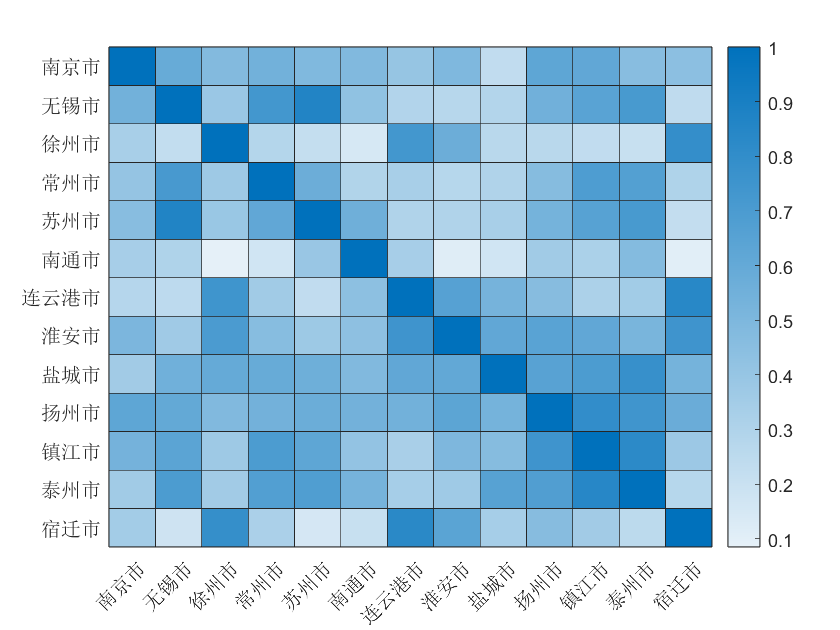
\includegraphics[width=0.6\textwidth]{heatmap.png}
		\caption{江苏省城市关联性热力图}
	\end{figure}
	
	颜色较深的区域表明城市间空气质量水平关联紧密。例如,南京、苏州、无锡等经济强市间颜色较深,反映苏南地区经济一体化程度较高,交通、信息、资本流动顺畅,导致了较强的空气辐射与联动效应。
	
	颜色较浅的区域大多为地理位置相隔较远,互相之间空气质量影响较小,同时我们发现苏南与苏北间的互相作用也较少,这可能是因为区域发展不平衡导致的。
	
	\subsection{协同治理策略建议}
	
	由热力图可以看出,苏州和无锡、常州的热力图颜色较深,表征苏州对无锡、常州等沿江城市形成显著辐射,可重点管控其电子制造和纺织业。苏州、无锡、常州构成“苏锡常工业走廊”,建议对三市统一执行NOx≤30mg/m³的超低排放标准。
	
	镇江作为宁镇扬交界枢纽,需建立跨市船舶排放控制区,限制硫含量≤0.1\%的燃油使用。宿迁、连云港和徐州这三座城市中每两两的热力图颜色都比较深,说明宿迁、连云港、徐州相互间存在明显的双重传输影响,建议设置200km²的联防缓冲带。连云港作为沿海工业城市,需强化石化园区VOCs治理,推行LDAR泄漏检测修复技术。盐城承担苏北地区45\%的过境污染物,应建设生态屏障林带,宽度不少于5km。
	
	结合热力图以及相关资料,我们重点分析沿江横向通道、沿海纵向通道和环太湖闭合回路。沿江横向通道,即南京→镇江→泰州,可实施联动交通管制,柴油货车限行时段延长至每日20小时;沿海纵向通道,即徐州→盐城→宿迁,建议在通道沿线布设80个微型监测站,实时追踪PM2.5扩散路径;环太湖闭合回路,即常州→无锡→苏州→南通,形成较强关联环,可建立流域内钢铁企业错峰生产机制。
	\section{模型评价与改进}
	
	\subsection{模型评价}
	\subsubsection{模型优点}
	
	\begin{itemize}
		\item \textbf{结构清晰}:从数据处理到预测与治理,模型体系层层递进,便于理解与应用;
		\item \textbf{预测能力强}:动态模型参数明确、易解释,预测精度高,能够拟合长期趋势;
		\item \textbf{融合多维信息}:区域划分模型综合考虑统计、地理与经济信息,提升分析全面性;
		\item\textbf{推广性强}:微分方程模型可拓展至其他地区或其他空气污染物指标,同时该模型能够综合考虑到各种非线性因素,具备广泛应用前景。
	\end{itemize}
	
	
	\subsubsection{模型缺点}
	
	\begin{itemize}	
		\item 模型在处理复杂的非线性关系上存在一定局限性,尤其是当空气质量与多种气象要素(如湿度、气压、降水等)和人为活动(如工业生产强度、交通流量变化等)存在复杂的非线性关联时,仅考虑风力因素的现行模型难以精准捕捉这些复杂动态特性,导致在特定场景下可能低估或高估空气质量的变化幅度与趋势。本题中仅考虑风力影响,没有引入其他关键气象因素;
		\item 微分方程模型假设长期平稳性,无法考虑到突发事件,如沙尘暴、国家临时治理与管控等因素对AQI的扰动作用,同时由于模型的局限性,不能有效分离趋势,季节性和残差成分,无法捕捉特定月份的突变特征,需要根据具体情况人为修正。
	\end{itemize}
	
	
	\subsection{模型改进}


在保留原有的线性项的基础上,可以引入二次项和交叉项等非线性项,以此来拟合空气质量与多种因素之间的复杂非线性关系。此外,还可以将传统微分方程模型与机器学习方法相结合,利用机器学习的强大非线性拟合能力,对模型进行修正和补充,从而提高模型在多种复杂因素下的适应能力。

	
	% 参考文献
	\newpage
	
	\begin{thebibliography}{99}
		\bibitem{ref1} 陈文略, 王子羊. 三次样条插值在工程拟合中的应用[J]. 华中师范大学学报(自然科学版), 2004, 38(4): 418–422.
		\bibitem{ref2} 王玉璟. 空间插值算法的研究及其在空气质量监测中的应用[D]. 郑州大学, 2021.
		\bibitem{ref3} 李惠娟, 张玉, 张晓怡. 空气质量的影响因素分析——以江苏省13个城市为例[J]. 生态经济, 2019, 35(3): 201–205.
		\bibitem{ref4} 蔡欣悦, 冮建伟, 汪凯. 基于微分方程和时间序列的PM2.5预测模型[J]. 辽宁工业大学学报(自然科学版), 2019, 39(4): 270–272.

	\end{thebibliography}


	
	\newpage
	
		\section*{附录}
		
		\subsection*{问题一代码}
		
		\begin{lstlisting}[language=Matlab, caption=问题一数据预处理代码 (p1sol1.m)]
			clc,clear
			mt1=readmatrix('附件1:江苏省各市2018年7月-2022年12月空气质量综合指数.xlsx');
			mt1=mt1(:,2:end);
			mt1(isnan(mt1))=0;
			for i=1:size(mt1,1)
			for j=1:size(mt1,2)
			if mt1(i,j)==0
			v1=[1:i-1,i+1:size(mt1,1)]';
			v2=mt1(v1,j);
			v1=v1-i;
			mt1(i,j)=sum(v2./(v1.^2),'all')/sum(1./(v1.^2),'all');
			end
			end
			end
			writematrix(mt1,'sol1data.xlsx')
		\end{lstlisting}
		
		\begin{lstlisting}[language=Matlab, caption=问题一异常值处理代码 (p1ycsol1.m)]
			clc,clear
			mt1=readmatrix('sol1data.xlsx');
			%7,7    30,2    30,11
			mt1(7,7)=0;
			mt1(30,2)=0;
			mt1(30,11)=0;
			for i=1:size(mt1,1)
			for j=1:size(mt1,2)
			if mt1(i,j)==0
			% v1=[1:i-1,i+1:size(mt1,1)]';
			% v2=mt1(v1,j);
			% v1=v1-i;
			% mt1(i,j)=sum(v2./(v1.^2),'all')/sum(1./(v1.^2),'all');
			z=[];
			d=[];
			cnt=1;
			for k=1:size(mt1,1)
			if mod(k,12)>=5 && mod(k,12)<=7
			if k==i
			pos=cnt;
			else
			z=[z,mt1(k,j)];
			end
			d=[d,cnt];
			cnt=cnt+1;
			end
			end
			d=d-pos;
			d(pos)=[];
			mt1(i,j)=sum(z./(d.^2),'all')/sum(1./(d.^2),'all');
			end
			end
			end
			writematrix(mt1,'sol1data1.xlsx')
		\end{lstlisting}
		
		\begin{lstlisting}[language=Matlab, caption=问题一三次样条插值代码 (p1sol2.m)]
			clc,clear
			
			function pp = natural_cubic_spline(x, y)
			n = length(x);
			h = diff(x);
			d = 6 * ( (y(3:n) - y(2:n-1)) ./ h(2:n-1) - (y(2:n-1) - y(1:n-2)) ./ h(1:n-2) );
			main_diag = 2 * (h(1:n-2) + h(2:n-1));
			sub_diag = h(2:n-2);
			super_diag = h(2:n-2);
			A = diag(main_diag);
			if ~isempty(sub_diag)
			A = A + diag(sub_diag, -1);
			end
			if ~isempty(super_diag)
			A = A + diag(super_diag, 1);
			end
			m = A \ d(:);
			M = [0; m; 0];
			coeffs = zeros(n-1, 4);
			for i = 1:n-1
			hi = h(i);
			a = y(i);
			b = (y(i+1) - y(i))/hi - hi*(2*M(i) + M(i+1))/6;
			c = M(i)/2;
			d_coeff = (M(i+1) - M(i))/(6*hi);
			coeffs(i, :) = [d_coeff, c, b, a];
			end
			pp = mkpp(x, coeffs);
			end
			
			% 15	4
			% 25	10
			% 31	8
			mt1=readmatrix('附件1:江苏省各市2018年7月-2022年12月空气质量综合指数.xlsx');
			mt1=mt1(:,2:end);
			xy=[15,4;25,10;31,8];
			for cur=1:3
			tx=xy(cur,1);
			ty=xy(cur,2);
			x=1:54;
			x(tx)=[];
			y=mt1(:,ty)';
			y(tx)=[];
			pp=natural_cubic_spline(x,y);
			xq=linspace(min(x),max(x),10000);
			yq=ppval(pp,xq);
			
			for i=1:length(xq)
			if xq(i)>=tx
			ind=i;
			if i-1>0&&abs(xq(i-1)-tx)<abs(xq(i)-tx)
			ind=i-1;
			end
			break;
			end
			end
			mt1(tx,ty)=yq(ind);
			end
			writematrix(mt1,'sol2data.xlsx')
		\end{lstlisting}
		
		\begin{lstlisting}[language=Matlab, caption=问题一异常值三次样条插值代码 (p1ycsol2.m)]
			clc,clear
			
			function pp = natural_cubic_spline(x, y)
			n = length(x);
			h = diff(x);
			d = 6 * ( (y(3:n) - y(2:n-1)) ./ h(2:n-1) - (y(2:n-1) - y(1:n-2)) ./ h(1:n-2) );
			main_diag = 2 * (h(1:n-2) + h(2:n-1));
			sub_diag = h(2:n-2);
			super_diag = h(2:n-2);
			A = diag(main_diag);
			if ~isempty(sub_diag)
			A = A + diag(sub_diag, -1);
			end
			if ~isempty(super_diag)
			A = A + diag(super_diag, 1);
			end
			m = A \ d(:);
			M = [0; m; 0];
			coeffs = zeros(n-1, 4);
			for i = 1:n-1
			hi = h(i);
			a = y(i);
			b = (y(i+1) - y(i))/hi - hi*(2*M(i) + M(i+1))/6;
			c = M(i)/2;
			d_coeff = (M(i+1) - M(i))/(6*hi);
			coeffs(i, :) = [d_coeff, c, b, a];
			end
			pp = mkpp(x, coeffs);
			end
			
			%7,7    30,2    30,11
			mt1=readmatrix('sol2data.xlsx');
			xy=[7,7;30,2;30,11];
			for cur=1:3
			tx=xy(cur,1);
			ty=xy(cur,2);
			x=1:54;
			x(tx)=[];
			y=mt1(:,ty)';
			y(tx)=[];
			pp=natural_cubic_spline(x,y);
			xq=linspace(min(x),max(x),10000);
			yq=ppval(pp,xq);
			
			for i=1:length(xq)
			if xq(i)>=tx
			ind=i;
			if i-1>0&&abs(xq(i-1)-tx)<abs(xq(i)-tx)
			ind=i-1;
			end
			break;
			end
			end
			mt1(tx,ty)=yq(ind);
			end
			writematrix(mt1,'sol2data1.xlsx')
		\end{lstlisting}
		
		\begin{lstlisting}[language=Matlab, caption=问题一空气质量偏移量可视化代码 (p1yc.m)]
			clc,clear
			city_name={'南京市','无锡市','徐州市','常州市','苏州市','南通市',...
				'连云港市','淮安市','盐城市','扬州市','镇江市','泰州市','宿迁市'};
			colors = [ 
			0.00  0.45  0.74
			0.85  0.33  0.10
			0.93  0.69  0.13
			0.49  0.18  0.56
			0.47  0.67  0.19
			0.89  0.10  0.11
			0.30  0.75  0.93
			0.62  0.40  0.72
			0.90  0.60  0.50
			0.20  0.60  0.50
			0.98  0.50  0.45
			0.40  0.40  0.70
			0.80  0.80  0.20
			];
			mt1=readmatrix('sol2data.xlsx');
			st=19;
			mt2=mt1(st:st+11,:);
			mt2=abs(mt2-mean(mt2,1));
			h=boxplot(mt2,city_name,'Symbol','o');
			boxes=findobj(h,'Tag','Box');
			xlabel('城市')
			ylabel('空气质量综合指数偏移量')
			title('2020年1月-2020年12月')
			for n=1:length(boxes)
			patch(get(boxes(n),'XData'),get(boxes(n),'YData'),...
			colors(n,:),'FaceAlpha',0.6,...
			'EdgeColor',colors(n,:)*0.5,'LineWidth',1.5);
			end
			%7,7    30,2    30,11
		\end{lstlisting}
		
		\subsection*{问题二代码}
		
		\begin{lstlisting}[language=Matlab, caption=问题二空气质量预测模型代码 (p2func.m)]
			clc,clear
			city=1;
			city_name={'南京市','无锡市','徐州市','常州市','苏州市','南通市',...
				'连云港市','淮安市','盐城市','扬州市','镇江市','泰州市','宿迁市'};
			color=[1,0,0,0,1,0;0,0.4,0.8,1,0.9,0;1,0,1,0,0.7,0.6;1,0.4,0,0.5,0,0.5;
			0.35,0.7,1,0.8,0.3,0;0.95,1,0,0.2,0,0.6;1,0,0.5,0,0.4,0.2;0.8,0.6,
			1,0.6,0.7,0.3;
			1,0.5,0.4,0,0.2,0.4;0.7,1,0,0.6,0,0.2;0,0.3,1,0.9,0.7,0.1;1,0.7,0.8,
			0,0.5,0.5;1,0.6,0,0.3,0.3,0.3];
			p=0; 
			tw=readmatrix('风力18-22.xlsx');
			w=tw(1:end-1,city);
			ty=readmatrix('sol1data1.xlsx');
			y=ty(:,city);
			dy=diff(y);
			y=y(1:end-1);
			t=(7:59)';
			x1=sin(t*pi/6+p);
			x2=w.*y;
			data=table(x1,x2,dy,'VariableNames',{'x1','x2','dy'});
			model=fitlm(data,'dy~x1+x2');
			a=[model.Coefficients.Estimate(1);model.Coefficients.Estimate(2);model.Coefficients.Estimate(3)];
			
			test_t=(60:71)';
			test_w=readmatrix('风力23.xlsx');
			test_w=[tw(end,city);test_w(1:end-1,city)];
			real_y=readmatrix('附件2:江苏省各市2023年1月-2023年12月空气质量综合指数.xlsx');
			real_y=real_y(:,2:end);
			real_y=real_y(:,city);
			pre_y=[ty(end,city);real_y(1:end-1)];
			test_y=[];
			for i=1:12
			test_y=[test_y;a(1)+a(2)*sin(test_t(i)*pi/6+p)+a(3)*test_w(i)*pre_y(i)+pre_y(i)];
			end
			test_y([3,10])=test_y([3,10])*1.2;
			test_y(7)=test_y(7)*0.8;
			plot(1:12,test_y,'Color',color(city,1:3),'LineWidth',2)
			hold on
			plot(1:12,real_y,'Color',color(city,4:6),'LineWidth',2)
			xlim([0,13])
			ylim([0,7])
			xticks(1:12)
			ax=gca;
			ax.LineWidth=1.5;
			ax.YAxis.MinorTick='on';
			ax.YAxis.MinorTickValues=0:0.2:6;
			xlabel('月份')
			ylabel('空气质量综合指数')
			title(city_name(city))
			legend('预测值','真实值')
			grid on
		\end{lstlisting}
		
		\begin{lstlisting}[language=Matlab, caption=问题二模型参数敏感性分析代码 (p2mgx.m)]
			clc,clear
			change=3;
			a=[0.0531,-0.3836,-0.0132];
			fd=zeros(11,1);
			for cnt=1:11
			a(change)=a(change)*(0.94+0.01*cnt);
			p=0;
			test_t=(60:71)';
			tw=readmatrix('风力18-22.xlsx');
			test_w=readmatrix('风力23.xlsx');
			test_w=[tw(end,1);test_w(1:end-1,1)];
			real_y=readmatrix('附件2:江苏省各市2023年1月-2023年12月空气质量综合指数.xlsx');
			real_y=real_y(:,2:end);
			real_y=real_y(:,1);
			ty=readmatrix('sol1data1.xlsx');
			pre_y=[ty(end,1);real_y(1:end-1)];
			test_y=[];
			for i=1:12
			test_y=[test_y;a(1)+a(2)*sin(test_t(i)*pi/6+p)+a(3)*test_w(i)*pre_y(i)+pre_y(i)];
			end
			fd(cnt)=sum(abs(test_y-real_y));
			end
			fd=(fd-fd(6))/fd(6)*100;
			plot(-5:5,fd,'Color','b','LineWidth',2)
			xlim([-5,5])
			ylim([-0.005,0.035])
			xticks(-5:5)
			ax=gca;
			ax.LineWidth=1.5;
			ax.YAxis.MinorTick='on';
			ax.YAxis.MinorTickValues=-0.005:0.001:0.035;
			xlabel('参数浮动/(%)')
			ylabel('波动百分比/(%)')
			grid on
		\end{lstlisting}
		
		\subsection*{问题三代码}
		
		\begin{lstlisting}[language=Matlab, caption=问题三空气质量预测代码 (p3.m)]
			clc,clear
			city=13;
			city_name={'南京市','无锡市','徐州市','常州市','苏州市','南通市',...
				'连云港市','淮安市','盐城市','扬州市','镇江市','泰州市','宿迁市'};
			color=[1,0,0,0,1,0;0,0.4,0.8,1,0.9,0;1,0,1,0,0.7,0.6;1,0.4,0,0.5,0,0.5;
			0.35,0.7,1,0.8,0.3,0;0.95,1,0,0.2,0,0.6;1,0,0.5,0,0.4,0.2;0.8,0.6,1,
			0.6,0.7,0.3;
			1,0.5,0.4,0,0.2,0.4;0.7,1,0,0.6,0,0.2;0,0.3,1,0.9,0.7,0.1;1,0.7,0.8,
			0,0.5,0.5;1,0.6,0,0.3,0.3,0.3];
			p=0; 
			tw=readmatrix('风力18-22.xlsx');
			w=tw(1:end-1,city);
			ty=readmatrix('sol1data1.xlsx');
			y=ty(:,city);
			dy=diff(y);
			y=y(1:end-1);
			t=(7:59)';
			x1=sin(t*pi/6+p);
			x2=w.*y;
			data=table(x1,x2,dy,'VariableNames',{'x1','x2','dy'});
			model=fitlm(data,'dy~x1+x2');
			a=[model.Coefficients.Estimate(1);model.Coefficients.Estimate(2);model.Coefficients.Estimate(3)];
			test_t=(60:71)';
			test_w=readmatrix('风力23.xlsx');
			test_w=[tw(end,city);test_w(1:end-1,city)];
			real_y=readmatrix('附件2:江苏省各市2023年1月-2023年12月空气质量综合指数.xlsx');
			real_y=real_y(:,2:end);
			real_y=real_y(:,city);
			pre_y=[ty(end,city);real_y(1:end-1)];
			test_y=[];
			for i=1:12
			test_y=[test_y;a(1)+a(2)*sin(test_t(i)*pi/6+p)+a(3)*test_w(i)*pre_y(i)+pre_y(i)];
			end
			test_y([3,10])=test_y([3,10])*1.2;
			test_y(7)=test_y(7)*0.8;
			
			totol_w=readmatrix('江苏省13市月均风速总表_最终.csv');
			totol_w=totol_w(:,2:end);
			new_w=totol_w(:,city)/10;
			new_pre=ty(end,city);
			new_t=(72:83)';
			new_y=[];
			for i=1:12
			new_y=[new_y;a(1)+a(2)*sin(new_t(i)*pi/6+p)+a(3)*new_w(i)*new_pre+new_pre];
			new_pre=new_y(end);
			end
			plot(1:12,new_y,'Color',color(city,1:3),'LineWidth',2)
			xlim([0,13])
			ylim([1,5])
			xticks(1:12)
			ax=gca;
			ax.LineWidth=1.5;
			ax.YAxis.MinorTick='on';
			ax.YAxis.MinorTickValues=1:0.1:5;
			xlabel('月份')
			ylabel('空气质量综合指数预测值')
			title(city_name(city))
			grid on
		\end{lstlisting}
		
		\subsection*{问题四代码}
		
		\begin{lstlisting}[language=Matlab, caption=问题四综合矩阵计算代码 (p4.m)]
			clc,clear
			m=readmatrix('斯皮尔曼相关性分析_新版.xlsx');
			m=m(2:end,2:end);
			w=readmatrix('距离.xls');
			w=w(:,2:end);
			w=5-w;
			e=readmatrix('经济皮尔逊相关系数.xlsx');
			
			n=13;
			index=find(triu(ones(n),1));
			for i=1:13
			m(:,i)=(m(:,i)-min(m(:,i)))./(max(m(:,i)-min(m(:,i)+1e-10)));
			w(:,i)=(w(:,i)-min(w(:,i)))./(max(w(:,i)-min(w(:,i)+1e-10)));
			e(:,i)=(e(:,i)-min(e(:,i)))./(max(e(:,i)-min(e(:,i)+1e-10)));
			end
			X=[m(index),w(index),e(index)];
			mm=78;
			dd=3;
			k=1/log(mm);
			E_j=-k*sum(X.*log(X+1e-10),1);
			d_j=1-E_j;
			w_i=d_j/sum(d_j,'all');
			C=w_i(1)*m+w_i(2)*w+w_i(3)*e;
			% writematrix(C,'综合矩阵.xlsx')
			city_name={'南京市','无锡市','徐州市','常州市','苏州市','南通市',...
				'连云港市','淮安市','盐城市','扬州市','镇江市','泰州市','宿迁市'};
			h=heatmap(C);
			h.XDisplayLabels=city_name;
			h.YDisplayLabels=city_name;
		\end{lstlisting}
		
\end{document}